%
% This template has been created by Theo J. Mertzimekis, PhD
% It can be modified freely to meet your needs.
% Help in using this thesis can be found here:
% http://users.uoa.gr/~tmertzi/LaTeX
%
% As a minimal credit to the creator, please do not remove the lines above
%

\documentclass[11pt]{report}

\usepackage{shellesc}

% some more
\usepackage{rotating}
\usepackage{graphicx}
\usepackage{lscape}
% \usepackage{ulem}
% package to highlight code
\usepackage[]{minted}
\usemintedstyle{vs}
\setminted{frame=single, framesep=2mm}
\usepackage{xcolor}
\colorlet{codecolor}{black!30}
\newcommand{\codebox}[1]{%
  \colorbox{codecolor}{\ttfamily \detokenize{#1}}%
}
% package to activate greek language - the sequence languages appear below is IMPORTANT!!!
%
% use only one of the two options below, depending on the language you want to use.
% also see instructions in line 75
%
\usepackage[greek,english]{babel} % use this line if greek version is desired
%\usepackage[english,greek]{babel} % use this line if english version is desired

\usepackage{varioref,multicol}
\usepackage{comment}
% package to handle graphics
\usepackage{graphicx}
% package for long tables, exceeding one single page
\usepackage{longtable}
% packages to handle multiple figures in a minipage
\usepackage{caption,subcaption}
% package to extend math capabilities
\usepackage{amsmath,amssymb,isotope}
\usepackage[version=4]{mhchem}
% package to include code listings
\usepackage{listings}
%package to activate XeTeX font manager
\usepackage{fontspec}
\usepackage{csquotes}
%Imports biblatex package
\usepackage{biblatex} 
%Import the bibliography file
\addbibresource{bibliography.bib} 

\usepackage{multirow}


% DOCUMENT LAYOUT
\usepackage{geometry} 
\geometry{a4paper,textwidth=150mm,textheight=220mm,marginparsep=4pt}
\setlength\parindent{8mm}
\setlength\parskip{3mm}

% FONTS
\usepackage{xunicode}
\usepackage{xltxtra}
\usepackage{xcolor}
\usepackage{noto} % --> Use Google Noto font to fix some characters when standard fonts (Times etc) are used
\defaultfontfeatures{Mapping=tex-text} % converts LaTeX specials (``quotes'' --- dashes etc.) to unicode
%\setromanfont{Times New Roman}
%\setsansfont{Arial}
%\setmonofont{Courier New}
%\setmainfont{Times New Roman} % You can set your main font here, if Google Noto is not chosen
\usepackage[skip=0pt]{caption}


% ---- CUSTOM AMPERSAND
\newcommand{\amper}{{\fontspec[Scale=.95]{Gentium Italic}\selectfont\itshape\&}}

% package to handle line spacing
\usepackage{setspace}
\renewcommand{\arraystretch}{1.25}

% HEADINGS
\usepackage{sectsty} 
\usepackage[normalem]{ulem} 
\sectionfont{\rmfamily\mdseries\upshape\Large}
\subsectionfont{\rmfamily\bfseries\upshape\normalsize} 
\subsubsectionfont{\rmfamily\mdseries\upshape\normalsize} 

% PDF SETUP
% ---- FILL IN HERE THE DOC TITLE AND AUTHOR
\usepackage[unicode,driverfallback=dvipdfmx, bookmarks, colorlinks, breaklinks, pdftitle={Ανάλυση C\#, Μεταγλωττιστές}]{hyperref}  
\hypersetup{linkcolor=blue,citecolor=blue,filecolor=black,urlcolor=blue} 

% package for fancy style headers and footers
%\usepackage{fancybox}

% redefine bullet symbols and section style
\renewcommand\thesection{\arabic{section}}
\setcounter{tocdepth}{2}
% \renewcommand{\labelitemi}{$\blacktriangleright$}
\renewcommand{\labelitemii}{$\bullet$}

% if GREEK is wanted, leave lines 78 and 103 as is.
% else remove lines 78-103
% change captions especially for greek language - if the document is in ENGLISH, they should vanish
\addto\captionsenglish{%
  \renewcommand\prefacename{Πρόλογος}%
  \renewcommand\refname{Αναφορές}%
  \renewcommand\abstractname{Περίληψη}%
  \renewcommand\bibname{Βιβλιογραφία}%
  \renewcommand\chaptername{Άσκηση}%
  \renewcommand\appendixname{Παράρτημα}%
  \renewcommand\contentsname{Περιεχόμενα}%
  \renewcommand\listfigurename{Κατάλογος Σχημάτων}%
  \renewcommand\listtablename{Κατάλογος Πινάκων}%
  \renewcommand\indexname{Ευρετήριο}%
  \renewcommand\figurename{Εικόνα}%
  \renewcommand\tablename{Πίνακας}%
  \renewcommand\partname{Μέρος}%
  \renewcommand\enclname{Συνημμένα}%
  \renewcommand\ccname{Κοινοποίηση}%
  \renewcommand\headtoname{Προς}%
  \renewcommand\pagename{Σελίδα}%
  \renewcommand\seename{βλέπε}%
  \renewcommand\alsoname{βλέπε επίσης}%
  \renewcommand\proofname{Απόδειξη}%
  \renewcommand\glossaryname{Γλωσσάρι}%
  \renewcommand\listingscaption{Κώδικας}%
  }

\newcommand*{\fullwidthimage}{0.94\textwidth}

%% hide default chapter titles
\usepackage{titlesec}
\titleformat{\chapter}{}{}{0em}{\bf\LARGE}
  
\usepackage{xgreek} %% this is to load greek hyphenation, remove if english is the basic language

%%%%%%%%% END OF PREAMBLE %%%%%%%%%%%%

\begin{document}

\setlanguage{greek} %% this is to activate greek hyphenation, remove if english is the basic language
% \pagenumbering{roman}


% make title out of \author, \title, \date  specified in the preamble
\begin{titlepage}
%
%
\begin{figure*}[ht]

\includegraphics[scale=0.6]{images/UOA_LOGO.png}
\end{figure*}


\vspace{10mm}
\hbox{ % Horizontal box
\hspace*{0.02\textwidth} % Whitespace to the left of the title page
\rule{1.5pt}{0.80\textheight} % Vertical line
\hspace*{0.02\textwidth} % Whitespace between the vertical line and title page text
\parbox[b]{0.95\textwidth}{ % Paragraph box which restricts text to less than the width of the page


{\large \textsc{Μεταγλωττιστές Κ31}}\\[\baselineskip] % Tagline or further description
{\noindent\Large\bfseries
Ανάλυση της γλώσσας C\#
} % Title
\\[2\baselineskip]

\includegraphics[scale=0.3]{images/OIP.jpeg}
\\[2\baselineskip]
{\Large Άγγελος Παπανικολάου} 
\\[0.10\baselineskip] 
ΑΜ 1115201800153
\\[1\baselineskip] % Author name

{\Large Δημήτριος Φωτόπουλος} 
\\[0.10\baselineskip] 
ΑΜ 1115202000292
\\[1\baselineskip] % Author name

{\Large Ζήσης Καμμάς} 
\\[0.10\baselineskip] 
ΑΜ 1115202000290
\\[2\baselineskip] % Author name

{\em Διδάσκων:}\\[0.25\baselineskip]
{\large Αθανάσιος Ανδρούτσος}
\\[1\baselineskip]


\vspace{0.05\textheight} % Whitespace between the title block and the publisher
{\noindent Αθήνα, Μάιος 2024}\\[\baselineskip] % Space and Time
}}
%
%
\end{titlepage}
% include the abstract, written in a separate file called thesis_abstract.tex

% \pagenumbering{arabic}
\setcounter{page}{1}

% Create table of contents - not mandatory
\tableofcontents
\newpage

% include files with content. Changes the names according to your taste.

\section{Εισαγωγή}

\subsection{C\# Δημιουργία - Εξέλιξη}
\label{C Sharp}
% \begin{minipage}{\textwidth}
Η \textbf{C\#} είναι μία γλώσσα προγραμματισμού Η/Υ. Δημιουργήθηκε από την \textbf{Microsoft}. Το \textbf{2000} η Microsoft ανακοίνωσε την δημιουργία της πλατφόρμας .Net. Το\textbf{ 1999} , δηλαδή 1 χρόνο πριν την δημιουργία του .Net, συγκροτήθηκε μία ομάδα με επικεφαλή τον Άντερς Χάιλσμπεργκ (ο οποίος θεωρείτε ο πατέρας της C \#) με σκοπό την δημιουργία μιας καινούργιας γλώσσας με όνομα \textbf{Cool} (C-like Object Oriented Language). Μέχρι τον Ιούλιο του 2000 που ανακοινώθηκε απο την Microsoft η πλατφόρμα .Net η γλώσσα είχε μετονομαστεί σε C\# στην οποία αργότερα εισήχθησαν οι βιβλιοθήκες της \textbf{ASP.NET}.

Η C\# όταν δημιουργήθηκε έμοιαζε πάρα πολύ με την \textbf{Java}. Προγραμματιστής της Java ονόματι \textbf{Τζέιμς Γκόσλινγκ} σχολίασε για την C\# ότι "Eίναι ίδια με την Java απλά χωρίς αξιοπιστία, παραγωγικότητα και ασφάλεια " αν και ο ιδρυτής της Άντερς Χάιλσμπεργκ υποστήριξε οτι δεν είναι κλώνος της Java αλλά ότι είναι πολύ κοντά στην C++. Με την κυκλοφορία της C\# 2.0 τον Νοέμβριο 2005 η Java και η C\# άρχισαν να απομακρύνονται προγραμματιστικά με σημαντική διαφορά στην υλοποίηση των \textbf{γενικών αντικειμένων}.

Ο κύριος σκοπός της C\# είναι να προσφέρει ένα ασφαλές, απλό, αλλά ισχυρό περιβάλλον για την ανάπτυξη λογισμικού που εκτελείται κυρίως στο .NET Framework της Microsoft. Η C\# σχεδιάστηκε για να είναι εύχρηστη για τους προγραμματιστές που ήδη γνωρίζουν C++ ή Java, προσφέροντας μια σύγχρονη γλώσσα με πλούσιες δυνατότητες αποδοτικότητας και ασφάλειας.

Παρέχει εργαλεία για την ανάπτυξη εφαρμογών Windows, Web services, διαδικτυακές εφαρμογές μέσω ASP.NET, καθώς και για εφαρμογές για κινητά και cloud. Επιπρόσθετα, η C\# υποστηρίζει σύγχρονες προγραμματιστικές αρχές και παραδείγματα, όπως η ενθυλάκωση, η κληρονομικότητα και η πολυμορφία, ενώ παράλληλα διαθέτει αυστηρό έλεγχο τύπων και αυτόματη διαχείριση μνήμης για την αποφυγή σφαλμάτων, όπως διαρροές μνήμης και άλλα.
% \end{minipage}

\begin{table}[h]
\centering
\label{my-label}
\resizebox{1.1\textwidth}{0.12\textheight}{%
\begin{tabular}{|l|l|l|l|l|l|l|}
\hline
\multicolumn{1}{|c|}{Έκδοση} & \multicolumn{3}{c|}{Γλώσσα Προγραμματισμού} & Ημερομηνία & \.NET Framework & Visual Studio \\ \cline{2-4}
 & ECMA & ISO/IEC & Microsoft &  &  &  \\ \hline
C\# 1.0 & Δεκέμβριος 2002 & Απρίλιος 2003 & Ιανουάριος 2002 & Ιανουάριος 2002 & .NET Framework 1.0 & Visual Studio .NET 2002 \\ \hline
C\# 1.2 & Δεκέμβριος 2002 & Απρίλιος 2003 & Οκτώβρης 2003 & Απρίλιος 2003   & .NET Framework 1.1 & Visual Studio .NET 2003 \\ \hline
C\# 2.0 & Ιούνιος 2006 & Σεπτέμβριος 2006 & Σεπτέμβριος 2005 & Νοέμβριος 2005 & .NET Framework 2.0 & Visual Studio 2005 \\ \hline
C\# 3.0 & \multicolumn{2}{c|}{Κανένα} & Αύγουστος 2007 & Νοέμβριος 2007 & .NET Framework 2.0/3.0/3.5 & Visual Studio 2008/2010 \\ \hline
C\# 4.0  & \multicolumn{2}{c|}{Κανένα} & Απρίλιος 2010 & Απρίλιος 2010 & .NET Framework 4 & Visual Studio 2010 \\ \hline
C\# 5.0  & \multicolumn{2}{c|}{Κανένα} & Ιούνιος 2013 & Αύγουστος 2012 & .NET Framework 4.5 & Visual Studio 2012/2013 \\ \hline
C\# 6.0  & \multicolumn{2}{c|}{Κανένα} & \multicolumn{2}{c|}{Κατάσταση: Δεν έχει κυκλοφορήσει ακόμα} & .NET Framework 4.6 & Visual Studio 2015 \\ \hline
\end{tabular}%
}
\end{table}

Ο παραπάνω πίνακας δείχνει την εξέλιξη της\textbf{ C\#} κατά τα χρόνια καθώς και τις συμβατότητες με \textbf{.Net Framework} και \textbf{Visual Studio}.



\textit{Το ECMA και το ISO/IEC είναι δύο σημαντικοί διεθνείς οργανισμοί που συμβάλλουν στην τυποποίηση διάφορων τεχνολογικών και βιομηχανικών προδιαγραφών, συμπεριλαμβανομένων των γλωσσών προγραμματισμού.}


\subsection{.Net Δημιουργία - Εξέλιξη}
\label{.NEt}
Η πλατφόρμα .Net της Microsoft είναι ένα ολοκληρωμένο αρχιτεκτονικό πλαίσιο και σύνολο τεχνολογιών που επιτρέπει την ανάπτυξη και την εκτέλεση πολλών τύπων εφαρμογών. Η πλατφόρμα υποστηρίζει παραδοσιακές εφαρμογές desktop-webpage εώς και μοντέρνες εφαρμογές κινητών και cloud-based εφαρμογές. Το .Net παρουσιάστηκε από τη Microsoft τον Ιούνιο του 2000, με την πρώτη έκδοση να κυκλοφορεί το \textbf{2002}. Η πρωτοβουλία .NET ήταν μέρος μιας μεγαλύτερης αλλαγής στην ανάπτυξη λογισμικού, με έμφαση στα Web services και την ανάπτυξη εφαρμογών μέσω ενός ενοποιημένου περιβάλλοντος. Η πρώτη έκδοση του .NET Framework περιλάμβανε το\textbf{ Common Language Runtime (CLR)}, το οποίο επέτρεπε την εκτέλεση προγραμμάτων γραμμένων σε διάφορες γλώσσες, καθώς και μια βιβλιοθήκη κλάσεων που παρείχε απαραίτητες λειτουργίες. Το \textbf{2005} ανακοινώθηκε η έκδοση \textbf{2.0} που περιλάμβανε σημαντικές βελτιώσεις, όπως την υποστήριξη για τον γενικευμένο προγραμματισμό, καλύτερη υποστήριξη για web εφαρμογές μέσω του ASP.NET και νέες τεχνολογίες για τη δημιουργία πιο δυναμικών web interfaces. 

Το \textbf{2008} αναβαθμίστηκε σε \textbf{.Net Framework 3.5} με την υποστήριξη του \textbf{Language Integrated Query (LINQ)} το οποίο επιτρέπει στους προγραμματιστές να γράφουν ερωτήματα δεδομένων στον κώδικα τους με πιο φυσικό τρόπο. Επίσης, περιελάμβανε ενσωματώσεις για την υποστήριξη των πλατφορμών web, όπως \textbf{AJAX} και \textbf{Web Services}. 

Το \textbf{2010} η αναβάθμιση σε \textbf{.NET Framework 4} έφερε την υποστήριξη για πιο προχωρημένες δυνατότητες, όπως βελτιωμένη παράλληλη επεξεργασία και καλύτερη διαχείριση μνήμης. Προστέθηκαν επίσης νέες δυνατότητες για τον προγραμματισμό των Windows Applications, όπως η βιβλιοθήκη Task Parallel Library. 

Το \textbf{2012} η αναβάθμιση σε \textbf{.NET Framework 4.5} παρουσίασε σημαντικές βελτιώσεις στην \textbf{ασφάλεια}, την \textbf{απόδοση}, και την ανάπτυξη web εφαρμογών, με περαιτέρω υποστήριξη για \textbf{HTML5} και \textbf{CSS3} στο ASP.NET.

Το \textbf{2015} η αναβάθμιση σε \textbf{.NET Framework 4.6} περιλάμβανε σημαντικές βελτιώσεις  στην υποστήριξη της γλώσσας C Sharp και το Visual Basic.

Το \textbf{2016} η Microsoft έκανε μια σημαντική αλλαγή πορείας με την κυκλοφορήσει του \textbf{ .NET Core RC1,} η οποία είναι μία νέα, cross-platform έκδοση του .NET που στοχεύει στην ανάπτυξη cloud-based και κινητών εφαρμογών. Το .NET Core σχεδιάστηκε να λειτουργεί σε διάφορα λειτουργικά συστήματα όπως \textbf{Windows}, \textbf{Linux},\textbf{MAC} και \textbf{macOS}, προσφέροντας τη δυνατότητα ανάπτυξης εφαρμογών με μεγάλη ευελιξία και προσβασημότητα. (Μέχρι τότε το .NET λειτουργούσε σε Windows)
\\[5\baselineskip]

Τα επόμενα χρόνια η Microsoft εστίασε στην αναβάθμιση του \textbf{.Net Core} ώστε να γίνει πιο ελκυστικό από τους προγραμματιστές με περισσότερες βιβλιοθήκες, καλύτερη απόδοση και νέες δυνατότητες.


\begin{table}[h]
    \centering
    \resizebox{1.1\textwidth}{0.12\textheight}{%
    \begin{tabular}{|l|l|l|l|l|l|l|l|l|l|l|l|l|l|l|l}
        \hline
        \textbf{Version} & \textbf{Released} & \textbf{Edition} & \textbf{Published}\\ \hline
        .NET Core RC1 & November 2015 & First & March 2016\\ \hline
        .NET Core 1.0 & June 2016 &  & \\ \hline
        .NET Core 1.1 & november 2016 &  & \\ \hline
        .NET Core 1.0.4 and .NET Core 1.1.1 & March2017 & Second & March 2017\\ \hline
        .NET Core 2.0 & August 2017 &  & \\ \hline
        .NET Core for UWP in Windows 10 Fall Creator Update & Octomber 2017 & Third & November 2017 \\ \hline
        .NET Core 2.1 (LTS) & May 2018 &  & \\ \hline
        .NET Core 2.2 (Current) & December 2018 &  & \\ \hline
        .NET Core 3.0 (Current) & September 2019 & Fourth & October 2019 \\ \hline
        .NET Core 3.1 (LTS) & December 2019 &  & \\ \hline
        Blazor WebAssembly 3.2(Current) & May 2020 &  & \\ \hline
        .NET 5.0 (Current) & November 2020 & Fifth & November 2020 \\ \hline
        .NET 6.0 (LTS) & November 2021 & Sixth & November 2021 \\ \hline
        .NET 7.0 (Current) & November 2022 & Seventh & November 2022 \\ \hline
        .NET 8.0 (LTS) & November 2023 & Eighth & November 2023 \\ \hline
    \end{tabular}
    }
    \label{tab:my_label}
\end{table}

\textbf{Παρακάτω ενδεικτικά  μερικές Γλώσσες Προγραμματισμού που υποστηρίζονται από το .Net}

\begin{enumerate}
    \item C\#
    \item Visual Basic .NET (VB.NET)
    \item F\#
    \item C++/CLI
    \item IronPython 
    \item IronRuby
    \item Boo
    \item PowerShell
    \item ASP.NET
    \item JScript.NET
    \item Unity
    \item Nemerle 
\end{enumerate}







\section{Εγκατάσταση C\#}

\subsection{Visual Studio}
\label{Visual Studio}
\setlength{\parindent}{10mm}

Tο \href{https://visualstudio.microsoft.com/downloads/}{\textbf{\uline{Visual Studio}}} είναι το IDE της Microsoft για το .NET για \textbf{Windows} και \textbf{Mac}.

\begin{enumerate}
    \item \textbf{Λήψη} Visual Studio από το Link παραπάνω.
    
    Επιλέξτε την έκδοση για το λογισμικό που σας ενδιαφέρει.
    \item Ανοίξτε το αρχείο .exe.

    \begin{figure*}[ht]
        \centering
        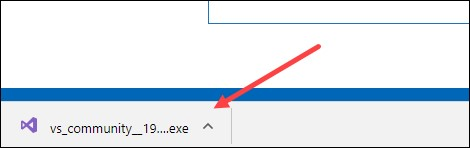
\includegraphics[scale=0.4]{images/inst1.jpg}
    \end{figure*}

    \item Στην επόμενη οθόνη, κάντε κλικ συνέχεια για να ξεκινήσετε την εγκατάσταση.

    \begin{figure*}[ht]
        \centering
        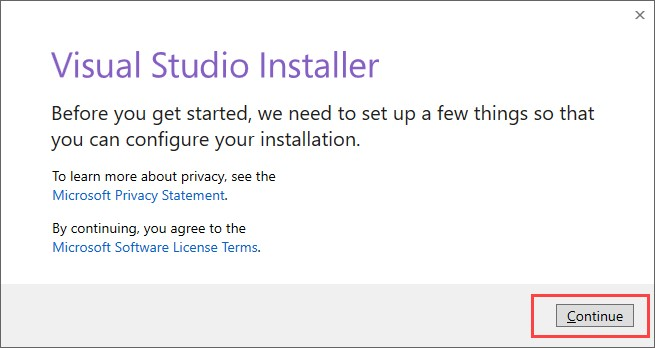
\includegraphics[scale=0.3]{images/inst2.jpg}
    \end{figure*}

    \item Αφήστε την εγκατάσταση να ολοκληρωθεί.

    \begin{figure*}[ht]
        \centering
        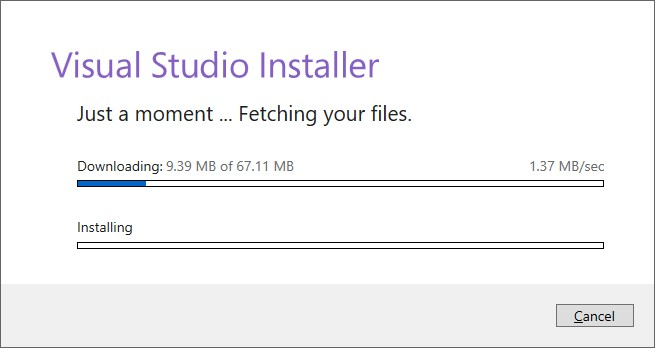
\includegraphics[scale=0.3]{images/inst3.jpg}
    \end{figure*}

    Visual Studio θα ξεκινήσει η λήψη των αρχικών αρχείων. Η ταχύτητα λήψης θα διαφέρει ανάλογα με τη σύνδεσή σας στο Διαδίκτυο.
    \\[4\baselineskip]
    \item Επιλέξτε την έκδοση λογισμικού που σας ενδιαφέρει.

    \begin{figure*}[ht]
        \centering
        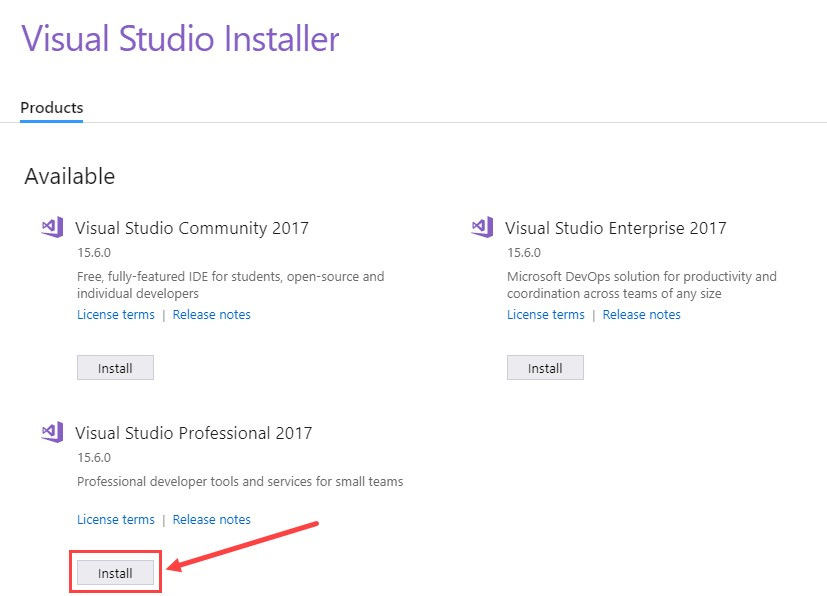
\includegraphics[scale=0.3]{images/inst4.jpg}
    \end{figure*}

    \item Επιλέξτε τα extensions που θα χρησιμοποιήσετε. Το .ΝΕΤ είναι επιτακτικό για C\#.

    \begin{figure*}[ht]
        \centering
        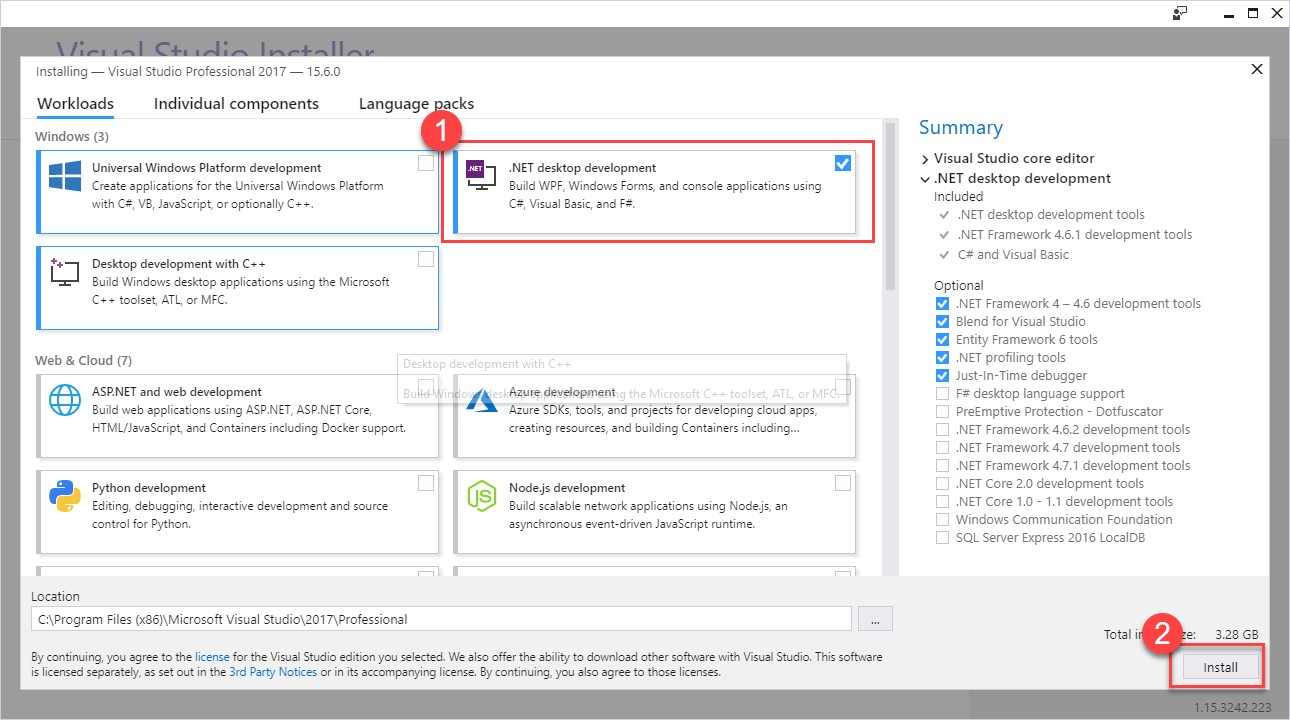
\includegraphics[scale=0.3]{images/inst5.jpg}
    \end{figure*}
    Πατήστε \textbf{Install} για να αρχίσει η εγκατάσταση.
    \\[8\baselineskip]
    
    \item Μόλις ολοκληρωθεί η εγκατάσταση των extensions χρειάζεται reboot.

    \begin{figure*}[ht]
        \centering
        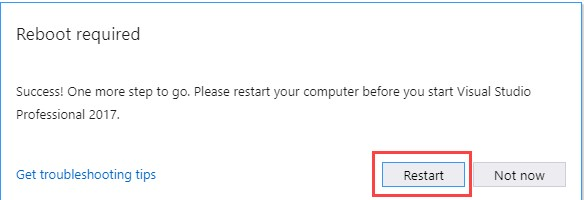
\includegraphics[scale=0.3]{images/inst7.jpg}
    \end{figure*}

    \item Ξεκινήστε την χρήση Visual Studio

    \begin{figure*}[ht]
        \centering
        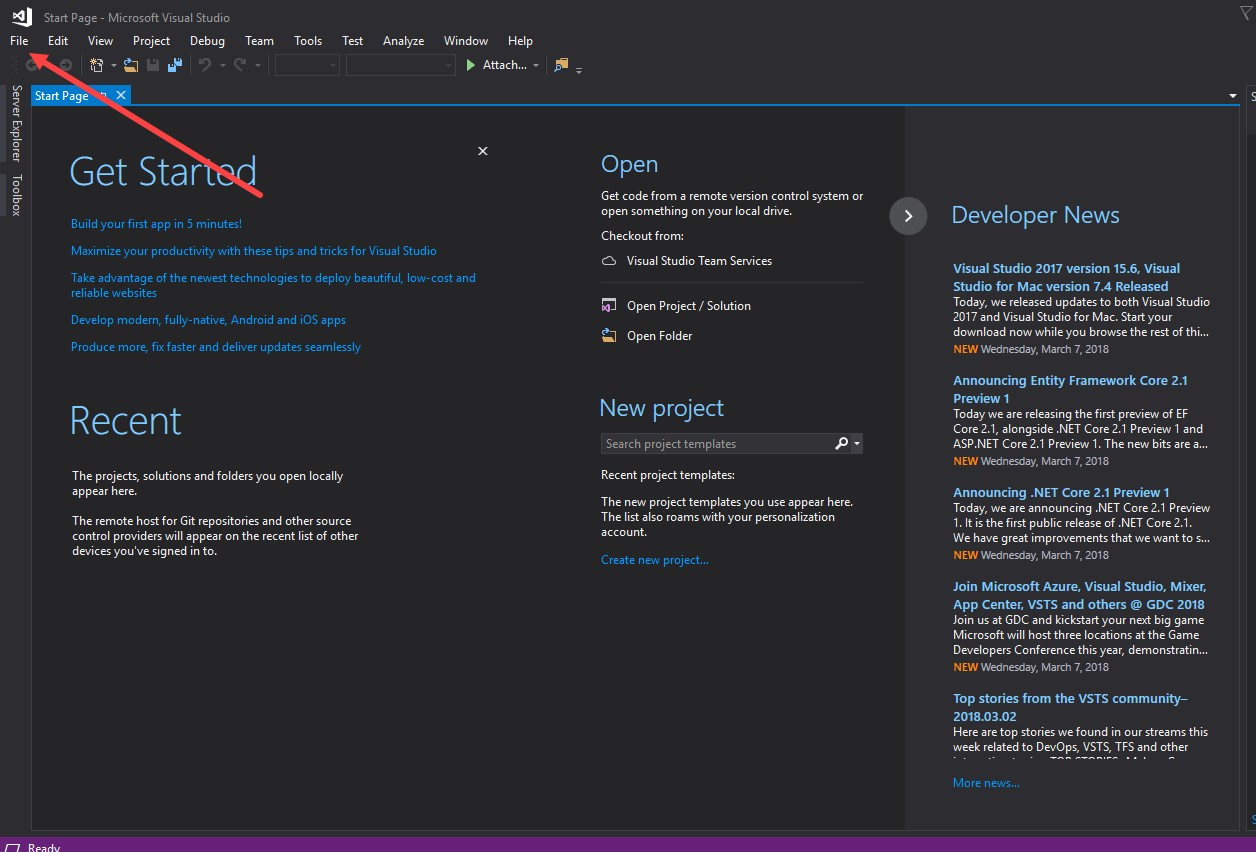
\includegraphics[scale=0.3]{images/inst8.jpg}
    \end{figure*}

    In Visual Studio IDE, μπορείτε να πλοηγηθείτε στο μενού \textbf{Αρχείο} για να δημιουργήσετε νέες εφαρμογές C\#.
\end{enumerate}

\textbf{Visual Studio Βασικά Xαρακτηριστικά.}

\begin{itemize}
    \item Δημιουργία μιας εφαρμογής σε οποιαδήποτε γλώσσα .Net.
    \item Δημιουργία οποιουδήποτε τύπου εφαρμογής.
    \item Εντοπισμός εφαρμογών εν κινήσει.
    \item Επεκτάσεις.
\end{itemize}
\

\subsection{Visual Studio Code}
\label{VS Code}
\setlength{\parindent}{10mm}
To \href{https://code.visualstudio.com/Download}{\textbf{\uline{Visual Studio Code}}} υποστηρίζεται και από \textbf{Windows},\textbf{Mac},\textbf{MacOs} και \textbf{Linux}.

\begin{enumerate}
    \item Κατεβάστε στον υπολογιστή σας το .ΝΕΤ της επιλογής σας \href{https://dotnet.microsoft.com/en-us/download/visual-studio-sdks}{\uline{εδώ}}.

    \item Ανοίξτε το .exe φάκελο που κατεβάσατε και ολοκληρώστε την εγκατάσταση του .ΝΕΤ. 

    \begin{figure*}[ht]
        \centering
        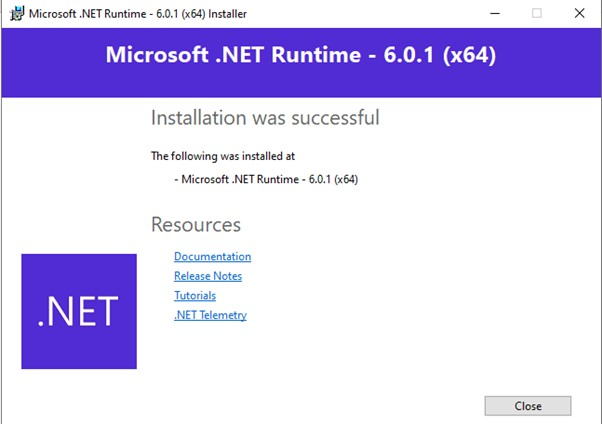
\includegraphics[scale=0.4]{images/instVSC1.jpg}
    \end{figure*}

    \item Ελέγξτε στο Command Channel αν η εγκατάσταση έγινε επιτυχώς πληκτρολογώντας \textbf{dotnet} - -\textbf{info}.

    \begin{figure*}[ht]
        \centering
        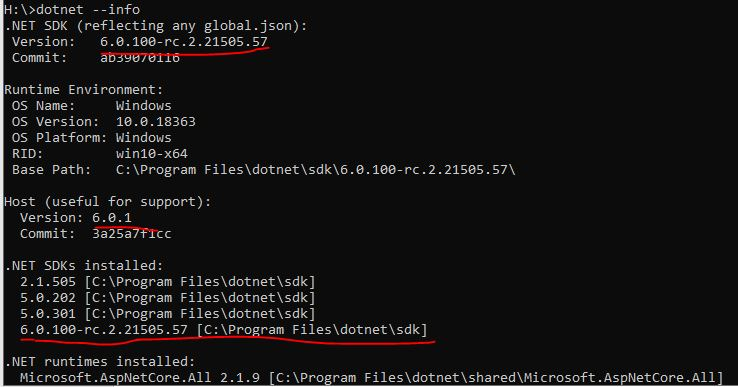
\includegraphics[scale=0.4]{images/instVSC2.jpeg}
    \end{figure*}

    Ελέγξτε ότι υπάρχουν τα αντίστοιχα υπογραμμισμένα στον υπολογιστή σας.
    \\[10\baselineskip]
    
    \item Κατεβάστε το VS Code ανάλογα με το λογισμικό του υπολογιστή σας \href{https://code.visualstudio.com/Download}{\uline{εδώ}}.

    \begin{figure*}[ht]
        \centering
        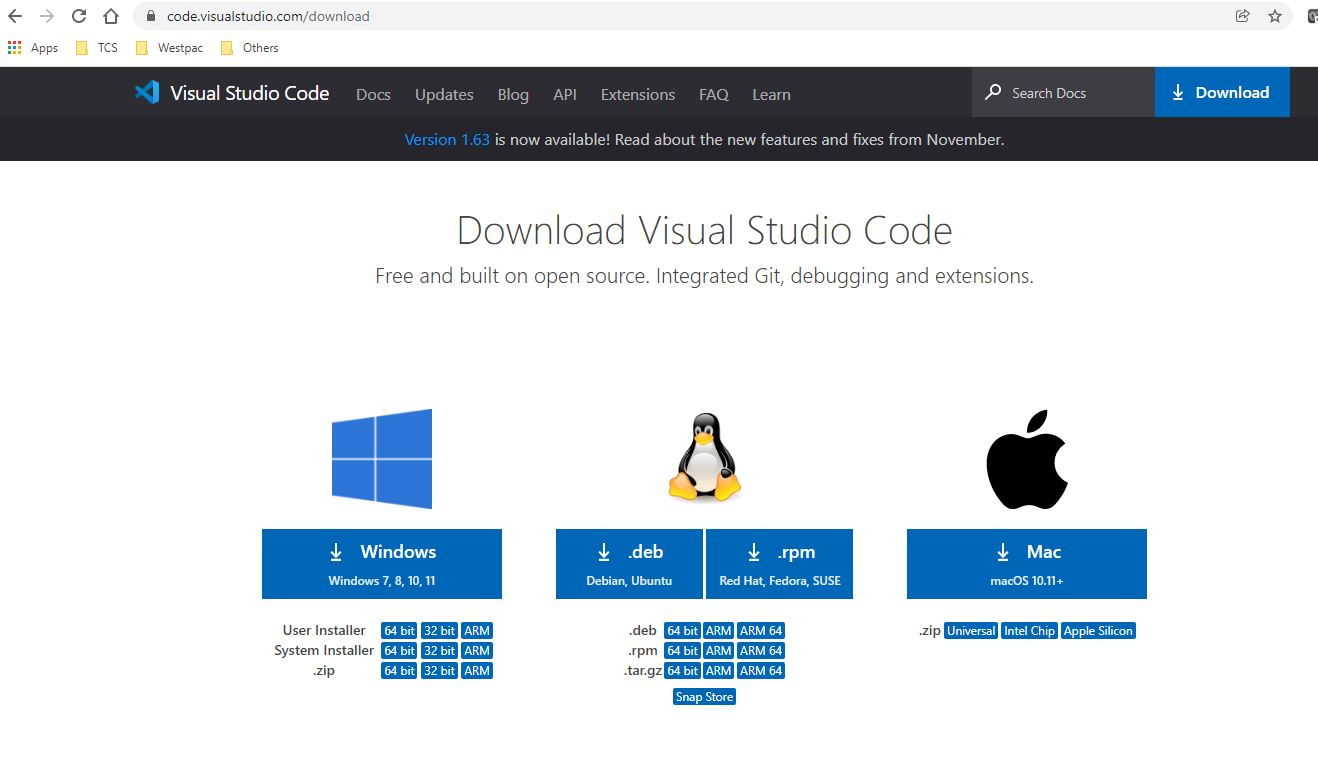
\includegraphics[scale=0.3]{images/instVSC3.jpeg}
    \end{figure*}

    \item Ανοίξτε τα Extensions του VS Code. \href{https://marketplace.visualstudio.com/VSCode}{\uline{εδώ}}

    Αναζητήστε και κατεβάσε την επέκταση για C\#. 

    \begin{figure*}[ht]
        \centering
        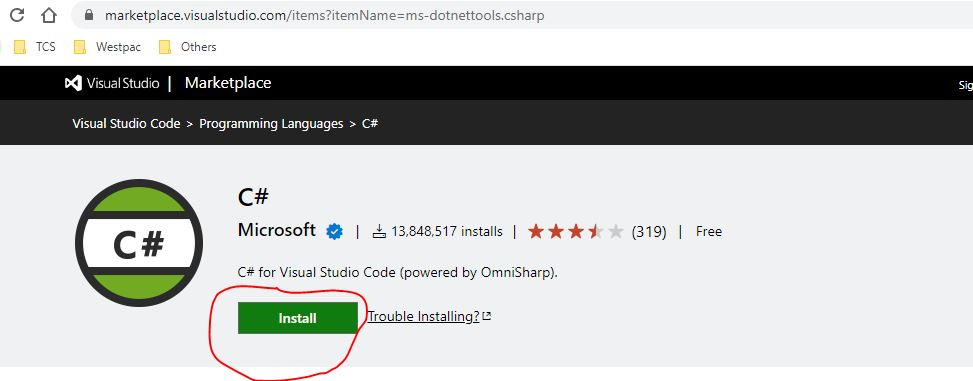
\includegraphics[scale=0.3]{images/instVSC4.jpeg}
    \end{figure*}

    Αυτό το βήμα μπορεί να γίνει και μέσα από το VS Code επιλέγοντας στο Menu Extension και αναζητώντας από εκεί την επέκταση για C\#.

    \item Ανοίξτε το VS Code στον υπολογιστή σας και δημιουργήστε εναν φάκελο Demo (ή μια ονομασία της επιλογής σας).Ανοίξτε αυτόν τον φάκελο ώστε να εμφαίζεται στα αριστερά του VS Code, στο μέρος που φαίνονται οι φάκελοι.
    \\[8\baselineskip]

    \item Ανοίξτε το terminal στο VS Code.
    \begin{figure*}[ht]
        \centering
        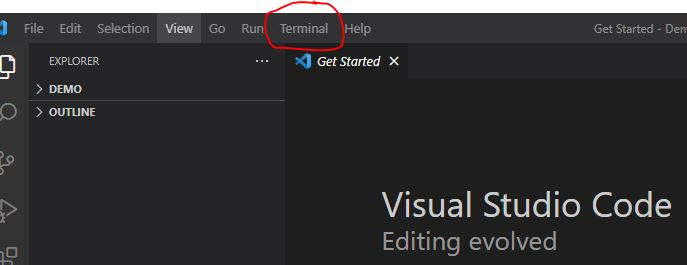
\includegraphics[scale=0.4]{images/instVSC5.jpeg}
    \end{figure*}

    \item Επιβεβαιώστε οτι βρίσκεστε στο σωστό Path αλλίως πλοηγηθείτε μέσω του terminal στο path που βρίσκεται το project (Demo) και πατήστε \textbf{dotnet new console}

    \begin{figure*}[ht]
        \centering
        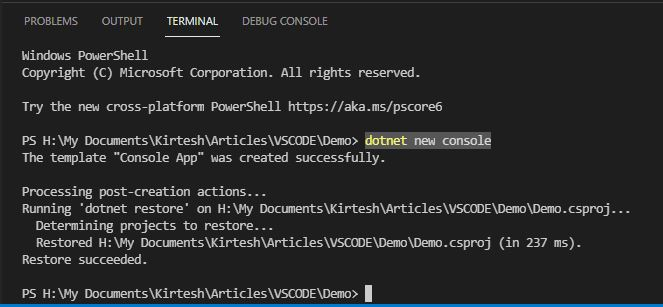
\includegraphics[scale=0.4]{images/instVSC6.jpeg}
    \end{figure*}

    \item Ελέγξτε ότι ο φάκελος Demo.csproj (εφόσον ονομάσατε το project Demo) περιλαμβάνει την έκδοση του .ΝΕΤ που εγκαταστήσατε όπως φαίνεται παρακάτω.

    \begin{figure*}[ht]
        \centering
        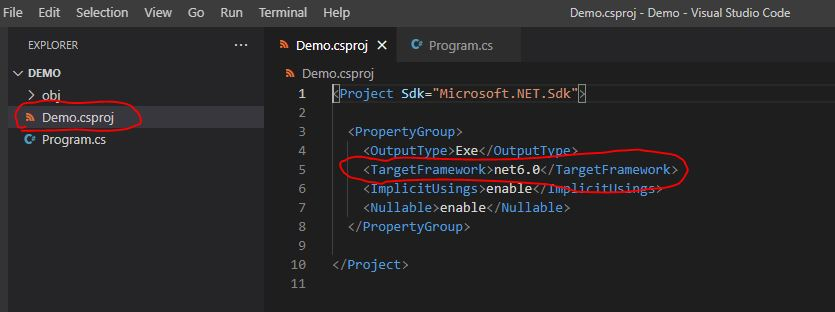
\includegraphics[scale=0.5]{images/instVSC7.jpeg}
    \end{figure*}

    Εφόσον όλα τα παραπάνω υλοποιήθηκαν σωστά. Γράψτε τον κωδικά σας στο program.cs.
    \\[8\baselineskip]

    \item Ο κώδικας σας θα εκτελεστεί πληκτρολογώντας στο terminal την εντολή \textbf{dotnet run}.

    \begin{figure*}[ht]
        \centering
        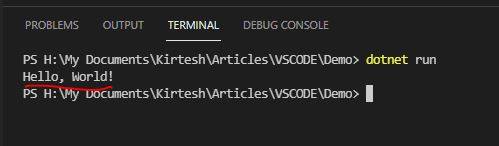
\includegraphics[scale=0.5]{images/instVSC8.jpeg}
    \end{figure*}
\end{enumerate}
\section{Κωδικας}

\subsection{Hello Wolrd - Το πρώτο πρόγραμμα σε C\#}
\label{Hello World}
\begin{listing}[htbp]
\begin{minted}[]{csharp}
using System;

namespace HelloWorld
{
    class Program
    {
        static void Main(string[] args)
        {
            Console.WriteLine("Hello World!");
        }
    }
}
\end{minted}
\caption{Το πρώτο πρόγραμμα σε C\#}
\label{HelloWorld}
\end{listing}

\codebox{Using System}: Η Γραμμή αυτή περιλαμβάνει τον χώρο ονομάτων (namespace) System, ο οποίος περιέχει θεμελιώδεις κλάσεις και βασικούς τύπους. Σε αυτή τη περίπτωση χρησιμοποιείται για την πρόσβαση στη κλάση Console, για λειτουργίες εισόδου - εξόδου.

\codebox{namespace HelloWord}: Τα namespaces παρουσιάζουν ομοιότητες με τα packages της Java. Είναι λογικοί containers, υπό την έννοια ότι οργανώνουν νοηματικά τις κλάσεις, χωρίς να αντιστοιχούν απαραίτητα σε φακέλους στο σύστημα.

\codebox{class Program}: Οι κλάσεις είναι containers για δεδομένα και μεθόδους, και αποτελούν θεμελιώδη δομικά στοιχεία του αντικειμενοστραφούς προγραμματισμού. ΚΑΘΕ γραμμή κώδικα που γράφεται σε C\#, πρέπει να βρίσκεται μέσα σε μια κλάση. Τη συγκεκριμένη κλάση την ονομάσαμε Program.

\codebox{static void Main}: Όπως και σε άλλες γλώσσες προγραμματισμού, η μέθοδος Main αποτελεί το σημείο εκκίνησης του προγράμματος. Με τον όρο static δηλώνεται ότι η μέθοδος ανοίκει στην ίδια την κλάση, και όχι σε κάποιο στιγμιότυπο αυτής. Με τον όρο void, η Main (και δηλαδή το πρόγραμμα) δεν επιστρέφει καμία τιμή. 

\codebox{Console.WriteLine(”Hello World!”)}: Τυπώνεται στην οθόνη η φράση "Hello World!". Η WriteLine είναι μια μέθοδος της κλάσης Console, η οποία λαμβάνει ως όρισμα ένα αλφαριθμητικό (string) και το τυπώνει στην κονσόλα, μαζί με έναν χαρακτήρα αλλαγής γραμμής.

Από το πρώτο κιόλας πρόγραμμα, μπορεί κάποιος να διακρίνει ομοιότητες με την Java: 

Η σύνταξη των δύο γλωσσών μοιάζει αρκετά, ιδίως στον τρόπο που συντάσσονται οι κλάσεις και οι μέθοδοι. Και οι δύο γλώσσες είναι αντικειμενοστραφείς, υποστηρίζοντας κλάσεις, αντικείμενα, κληρονομικότητα, πολυμορφισμό κ.α.

Η μέθοδος Main έχει παρόμοια σύνταξη και υπηρετεί τον ίδιο σκοπό. 

Standard Libraries: H C\# και η Java διαθέτουν μεγάλη ποικιλία από βιβλιοθήκες που παρέχουν ένα μεγάλο φάσμα από λειτουργίες. Στο πρόγραμμα Hello World, η "System.Console.WriteLine" της C\#, είναι η αντίστοιχη "System.out.println" της Java. 

\subsection{The Basics: Variables, methods, loops, if statements}
\label{Basics}
1. Οι μεταβλητές στη C\# δηλώνονται χρησιμοποιώντας τον τύπο δεδομένων ακολουθούμενο από το όνομα της μεταβλητής. Μπορούν να αρχικοποιηθούν κατά την δήλωση ή αργότερα στον κώδικα. Τα ονόματα ξεκινούν με γράμμα ή με κάτω παύλα \_ . Οι υπόλοιποι χαρακτήρες μπορούν να είναι γράμματα, αριθμοί, ή \_ . Η γλώσσα είναι case-sensitive (number != Number). 

\begin{listing}[htbp]
\begin{minted}[]{csharp}
int number;
string message = "Hello, world!";
bool isTrue = true;
double Number = 3.14;
\end{minted}
\caption{Δηλώσεις μεταβλητών}
\label{flagExec}
\end{listing}

2. Οι συναρτήσεις στη C\# ονομάζονται μέθοδοι. Δηλώνονται με τον τύπο δεδομένων της επιστρεφόμενης τιμής (void εάν δεν επιστρέφουν τιμή), ακολουθούμενο από το όνομα της μεθόδου και τις παραμέτρους.

\begin{listing}[htbp]
\begin{minted}[]{csharp}
// Defining a simple function
void PrintMessage(string message)
{
    Console.WriteLine(message);
}

// Calling the function
PrintMessage("This is a function call");
\end{minted}
\caption{Απλή συνάρτηση}
\label{flagExec}
\end{listing}

3. Δομές επανάληψης (loops). Προσφέρονται διάφοροι τύποι επαναλήψεων, όπως 'for', 'while' και 'do-while'. Η σύνταξή τους είναι όπως στις C/C++.

\begin{listing}[htbp]
\begin{minted}[]{csharp}
for (int i = 0; i < 5; i++)
{
    Console.WriteLine("Number: " + i);
}
\end{minted}
\caption{Βρόχος που τυπώνει τους αριθμούς 0 έως και 4}
\label{flagExec}
\end{listing}

4. Οι εντολές if-else, χρησιμοποιούνται και αυτές με τον ίδιο τρόπο όπως στις C/C++.

\begin{listing}[htbp]
\begin{minted}[]{csharp}

int grade = 7;
if (grade >= 5)
{
    Console.WriteLine("PASS");
}
else
{
    Console.WriteLine("FALL");
}
\end{minted}
\caption{Απλό if - else statement}
\label{flagExec}
\end{listing}

5. Όλοι οι τύποι που μπορούν να οριστούν στην γλώσσα δίνονται συγκεντρωτικά στην εικόνα \ref{fig:types} \cite{typesbook}.

\begin{figure}[h!]
  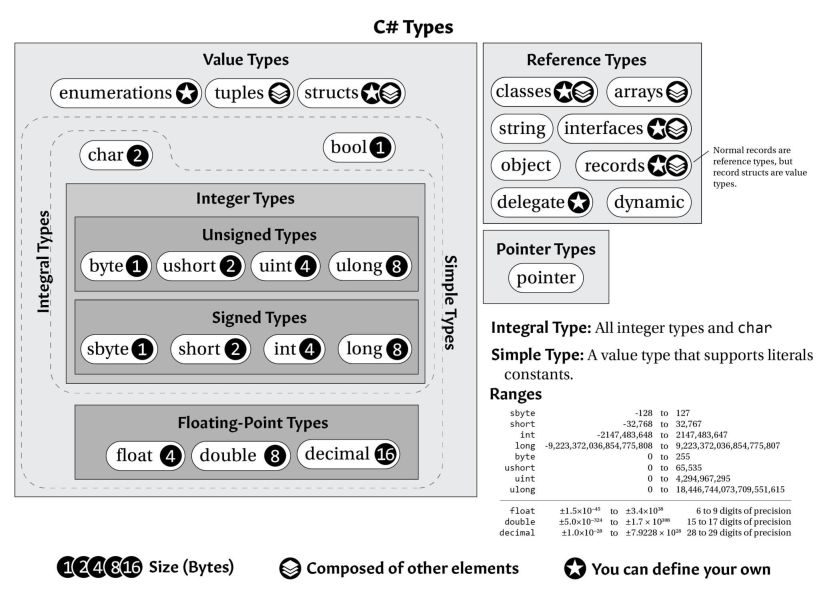
\includegraphics[width=\fullwidthimage]{images/csharptypes.jpg}
  \caption{Τύποι της C\#}
  \label{fig:types}
\end{figure}



\subsection{Implicit δήλωση μεταβλητών}
\label{implicitdeclaration}
Στη C\# παρέχεται η δυνατότητα να δηλωθούν μεταβλητές χωρίς να δηλωθεί ρητά και ο τύπος τους, όπως στο παράδειγμα του κώδικα \ref{implicitDeclaration}. Η implicit δήλωση μεταβλητών μπορεί να πραγματοποιηθεί με τρεις διαφορετικούς τρόπους, ανάλογα με τον βαθμό ελευθερίας.

Ο πρώτος τρόπος και πιο συνηθισμένος τρόπος είναι η χρήση της λέξης κλειδιού \codebox{var}. Με αυτό τον τρόπο συνεχίζει να εφαρμόζεται η στατική δήλωση των μεταβλητών. Ο μεταγλωττιστής της γλώσσας αποφασίζει τον καταλληλότερο τύπο για τη μεταβλητή σύμφωνα με την τιμή αρχικοποίησής της κατά τον χρόνο μεταγλώττισης, μην επιτρέποντας στη συνέχεια την αλλαγή του τύπου της μεταβλητής. Για το λόγο αυτό δεν είναι δυνατό να δηλωθεί μία μεταβλητή με τη χρήση της \codebox{var} χωρίς, ταυτόχρονα, να αρχικοποιηθεί.

Ο δεύτερος τρόπος είναι η χρήση της λέξης κλειδιού \codebox{dynamic}. Χρησιμοποιώντας της η μεταβλητή μπορεί να αλλάζει τύπο όσες φορές χρειάζεται, στα πρότυπα των scripting γλωσσών προγραμματισμού όπως η python και η javascript. Ο τύπος της μεταβλητής αποφασίζεται κατά τον χρόνο εκτέλεσης. Η δυνατότητα αυτή, όμως, έρχεται με ένα σχετικά μεγάλο κόστος εκτέλεσης.

Ο τρίτος τρόπος είναι η χρήση της λέξης \codebox{object}. Η γενική λέξη αντικειμένου της γλώσσας επιτρέπει στη μεταβλητή να πάρει οποιαδήποτε τιμή, δεδομένης της αντικειμενοστρέφειας της γλώσσας. Πρέπει, όμως, να σημειωθεί πως οι πιθανές μέθοδοι του τύπου της μεταβλητής δεν μπορούν να χρησιμοποιηθούν άμεσα, αλλά επιβάλλεται να γίνει casting. 

\begin{listing}[htbp]
\begin{minted}[]{csharp}
var staticVar = "compilers"; // string
staticVar = 10; // error

dynamic dynamicVar = "compilers"; // runtime string
Console.WriteLine(dynamicVar.Length); // 9
dynamicVar = 10; // ok

object objectVar = "compilers";
Console.WriteLine(objectVar.Length); // error
objectVar = 10; // ok
\end{minted}
\caption{Implicit δήλωση μεταβλητών}
\label{implicitDeclaration}
\end{listing}

\subsection{Classes - Objects}
\label{Classes - Objects}
Οι κλάσεις και τα αντικείμενα είναι οι δύο βασικές ιδέες του αντικειμενοστραφούς προγραμματισμού. Η διαφορά μεταξύ τους γίνεται εύκολα κατανοητή με την παρακάτω εικόνα.

\begin{table}[h]
    \centering
    \small{
    \begin{tabular}{|l|l|}
        \hline
        \textbf{Κλάση} & \textbf{Αντικείμενο} \\ \hline
        \multirow{3}{*}{Animal} & Cat \\ \cline{2-2}
        & Dog \\ \cline{2-2}
        & Snake \\ \hline
        \multirow{3}{*}{Car} & Toyota \\ \cline{2-2}
        & Hyundai \\ \cline{2-2}
        & Kia \\ \hline
    \end{tabular}
    }
    \label{tab:my_label}
\end{table}

Κλάση είναι το πρωτότυπο, η γενική ιδέα. Αντικείμενο είναι ένα στιμγιότυπο της κλάσης. Όταν ένα στιγμιότυπο μιας κλάσης δημιουργείται, αποκτά τα χαρακτηριστικά και τις μεθόδους αυτής. Τα πάντα στη C\# σχετίζονται με τις κλάσεις.

Για να δημιουργηθεί μια κλάση, χρησιμοποιείται η λέξη-κλειδή \codebox{class}. Για να δημιουργηθεί ένα αντικείμενο μιας κλάσης, χρησιμοποιείται η λέξη-κλειδί \codebox{new} ακολουθούμενο από το όνομα της κλάσης.

\begin{listing}[H]
\begin{minted}[]{csharp}
class Program
{
    internal class Animal
    {
        public int legsNum;
    }

    static void Main(string[] args)
    {
        // Creating a new instance of the Animal class
        Animal dog = new Animal();
        dog.legsNum = 4;
        
        // Another instance of the Animal class
        Animal snake = new Animal();
        snake.legsNum = 0;
        
        Console.WriteLine("Dog has {0} legs", dog.legsNum);
        Console.WriteLine("Snake has {0} legs" ,snake.legsNum);
    }
}
\end{minted}
\caption{Απλή κλάση}
\label{animal_simple}
\end{listing}

\subsection{Inheritance}
\label{inheritance}
Η κληρονομικότητα επιτρέπει την κατασκευή κλάσεων από κάποια υπάρχουσα κλάση και αποτελεί μία από τις βασικότερες λειτουργίες του αντικειμενοστραφούς προγραμματισμού.

Οι κλάσεις που κληρονομούν από κάποια άλλη ονομάζονται υποκλάσεις και έχουν διαθέσιμα όλα τα πεδία και τις μεθόδους της γονικής κλάσης, συμβάλλοντας στην επαναχρησιμοποίηση του κώδικα.

Συντακτικά, για να κληρονομήσει μία κλάση κάποια άλλη χρησιμοποιείται ο τελεστής \codebox{:}. Για παράδειγμα στον κώδικα \ref{inheritanceClasses} οι κλάσεις \codebox{Cat} και \codebox{Dog} κληρονομούν από την κλάση \codebox{Animal}.

Η κλήση του κατασκευαστή της γονικής κλάσης γίνεται με τη χρήση του κώδικα \codebox{: base(...)} αμέσως μετά τη δήλωση του κατασκευαστή της νέας κλάσης.

Οι κλάσεις \codebox{Cat} και \codebox{Dog} κληρονομούν και έχουν διαθέσιμα όλα τα μη ιδιωτικά πεδία και μεθόδους της \codebox{Animal}, όπως φαίνεται και κατά την εκτέλεσή τους στον κώδικα \ref{inheritanceExec}.

\begin{listing}[H]
\begin{minted}[]{csharp}
internal enum Family
{
    Canidae,
    Felidae
}

internal abstract class Animal
{
    private int _age = 0;
    public int Age => _age;
    public int Lifespan {get; }
    public Family Family { get; }
    protected Animal(Family family, int lifespan) 
        { Family = family; Lifespan = lifespan; }
    public void IncreaseAge() => _age++;
    public abstract void MakeSound();
    public bool IsAlive() => Age <= Lifespan;
}

internal class Cat : Animal
{
    public string Name { get; }
    public Cat(string name) : base(Family.Felidae, 18)
        { Name = name; }
    public override void MakeSound() => 
        Console.WriteLine("Meow meow!");
}

internal class Dog : Animal
{
    public string Name { get; }
    public Dog(string name) : base(Family.Canidae, 13)
        { Name = name; }
    public override void MakeSound() => 
        Console.WriteLine("Woof woof!");
}
\end{minted}
\caption{Κλάσεις με κληρονομικότητα}
\label{inheritanceClasses}
\end{listing}

Η τροποποίηση μεθόδων της γονικής κλάσης από τις υποκλάσεις γίνεται με τη χρήση της δεσμευμένη λέξης \codebox{override} ανάμεσα από τον access modifier και τον τύπο επιστροφής της μεθόδου. Για να είναι δυνατή η τροποποίηση μίας μεθόδου είναι απραίτητο αυτή να έχει δηλωθεί από τη γονική κλάση ως \codebox{abstract} ή \codebox{virtual}. Στην πρώτη περίπτωση η μέθοδος δεν υλοποιείται καθόλου από τη γονική κλάση, ενώ στη δεύτερη παρέχεται υλοποίηση αλλά η υποκλάση μπορεί να εφαρμόσει τη δική της. Έτσι, μέσω της κληρονομικότητας επιτυγχάνεται και ο πολυμορφισμός.

\begin{listing}[H]
\begin{minted}[]{csharp}
Animal dog = new Dog("Max");
Animal cat = new Cat("Dora");

dog.MakeSound();
cat.MakeSound();
Console.log($"{((Dog)dog).Name} " +
  $"{(dog.IsAlive() ? "is" : "is not")} alive.");
\end{minted}
\caption{Εκτέλεση κλάσεων με κληρονομικότητα}
\label{inheritanceExec}
\end{listing}

Όπως ισχύει και γενικότερα σε σχέση με την ορατότητα των πεδίων και των μεθόδων, οι δηλώσεις \codebox{private} διατίθενται αποκλειστικά στην ίδια την κλάση που τις δηλώνει, οι \codebox{protected} στην κλάση που κάνει τη δήλωση και τις υποκλάσεις τις, ενώ οι \codebox{public} είναι ορατές σε όλους.

Σημειώνεται πως στη C\# ενώ μία κλάση μπορεί να έχει όσες υποκλάσεις είναι επιθυμητό, κάθε υποκλάση μπορεί να έχει μία και μοναδική γονική κλάση. Αυτός ο περιορισμός δύναται σε να ξεπεραστεί σε ένα βαθμό με τη χρήση των \codebox{Interfaces} τα οποία επιτρέπουν πολλαπλή κληρονομικότητα.



\subsection{Reflection}
\label{reflection}
\titleformat{\chapter}{}{}{0em}{\bf\LARGE}

Η χρήση του reflection επιτρέπει την επισκόπηση και την τροποποίηση κλάσεων, πεδίων, μεθόδων και κατασκευαστών κατά τον χρόνο εκτέλεσης του προγράμματος.

Μετά την επιτυχή μεταγλώττιση του κώδικα κατασκευάζεται αυτόματα από τον μεταγλωττιστή ένα μπλοκ που ονομάζεται Assembly και περιέχει την ενδιάμεση γλώσσα και μεταδεδομένα.

Τα μεταδεδομένα αποτελούνται από πληροφορίες σχετικά με τις κλάσεις, τις μεθόδους, τους κατασκευαστές κτλ. Με το reflection γίνεται έλεγχος αυτών των μεταδεδομένων για την ανάκτηση πληροφοριών ενός assembly.

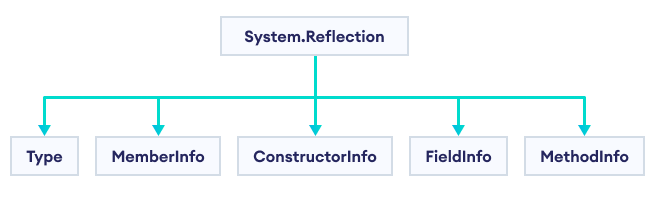
\includegraphics[width=\fullwidthimage]{code/Reflection/csharp-reflection-hierarchy.png}

Η βασική μέθοδος πρόσβασης στα μεταδεδομένα γίνεται με τη χρήση της κλάσης \codebox{Type}, η οποία παρέχει μεθόδους και ιδιότητες που δίνουν πληροφορίες για κάποιον τύπο.

Για παράδειγμα, για τις κλάσεις (\ref{inheritanceClasses}) του παραδείγματος της κληρονομικότητας (\ref{inheritance}), με reflection μπορεί να γίνει εξακρίβωση του τύπου της κάθε μεταβλητής όπως στον κώδικα \ref{reflectionInheritance}.

\begin{listing}[htbp]
\begin{minted}[]{csharp}
Animal dog = new Dog("Max");
Animal cat = new Cat("Dora");

Type type = dog.GetType();
Type type2 = cat.GetType();

Console.WriteLine(type);
Console.WriteLine(type2);
\end{minted}
\caption{Εξακρίβωση τύπου μεταβλητών της κλάσης του κώδικα \ref{inheritanceClasses}}
\label{reflectionInheritance}
\end{listing}

\begin{listing}[htbp]
\begin{minted}[]{csharp}
internal class NoChanging
{
    private string _shouldNotChange;
    public string ShouldNotChange => _shouldNotChange;

    public NoChanging(string shouldNotChange)
    {
        _shouldNotChange = shouldNotChange;
    }
}
\end{minted}
\caption{Κλάσης με private πεδίο και μέθοδο}
\label{reflectionClass}
\end{listing}

Σε άλλο παράδειγμα, για την κλάση του κώδικα \ref{reflectionClass}, μπορεί να γίνει απαρίθμηση των μεθόδων μίας κλάσης, όπως στο παράδειγμα του κώδικα \ref{reflectionProperties}.

\begin{listing}[htbp]
\begin{minted}[]{csharp}
NoChanging a = new NoChanging("First!");

var properties = a.GetType().GetProperties();

Console.WriteLine("Listing class properties...");
foreach (var property in properties)
{
    Console.WriteLine(property.Name, property.PropertyType);
}
\end{minted}
\caption{Απαρίθμηση μεθόδων}
\label{reflectionProperties}
\end{listing}

\newpage
Με reflection μπορούν τα τροποποιηθούν ακόμα και private πεδία μίας κλάσης όπως στο παράδειγμα \ref{reflectionChangePrivate}.

\begin{listing}[htbp]
\begin{minted}[]{csharp}
NoChanging a = new NoChanging("First!");

Console.WriteLine($"Initial value of private " +  
    $"field: {a.ShouldNotChange}");
Console.WriteLine($"Trying to change it...");

var str = a
    .GetType()
    .GetField("_shouldNotChange", 
        BindingFlags.NonPublic | BindingFlags.Instance);

str.SetValue(a, "Second!");

Console.WriteLine($"It changed(!!): {a.ShouldNotChange}");
\end{minted}
\caption{Τροποποίηση private πεδίου}
\label{reflectionChangePrivate}
\end{listing}



\subsection{Generics}
\label{generics}
Η χρήση των Generics επιτρέπει στην ίδια κλάση ή μέθοδο να χρησιμοποιείται με διαφορετικούς τύπους δεδομένων, διευκολύνοντας την επαναχρησιμοποίηση του κώδικα.

Για τη δήλωση μίας generic κλάσης χρησιμοποιούνται τα \codebox{<>} αμέσως μετά το όνομά της, όπως στο παράδειγμα του κώδικα \ref{genericsPersonClass}. Το \codebox{T} ανάμεσα στα \codebox{<>} ονομάζεται μεταβλητή τύπου. Η κλάση του κώδικα υποστηρίζει για το κάθε άτομο ένα Id οποιουδήποτε τύπου, πέρα από το όνομα και τον τίτλο του. Ο τύπος του Id ορίζεται κατά τη δήλωση ενός αντικειμένου και δεν μπορεί να αλλάξει κατά τον χρόνο εκτέλεσης. Σε περίπτωση που δοθεί διαφορετικός τύπος δεδομένων από αυτόν που ορίστηκε προκύπτει σφάλμα κατά τον χρόνο μεταγλώττισης του προγράμματος. 

\begin{listing}[htbp]
\begin{minted}[]{csharp}
internal class Person<T>
{
    private T _id;
    public T Id => _id;
    public string Name { get; set; }
    public string Title { get; set; }

    public Person(T id) { _id = id; }
    
    public Person(T id, string name, string title) : this(id)
    {
        Name = name; Title = title;
    }

    public override string ToString()
    {
        return $"Id: {_id}, Title: {Title}, Name: {Name}";
    }
}
\end{minted}
\caption{Κλάση με γενικό όρισμα}
\label{genericsPersonClass}
\end{listing}

Η χρήση μίας κλάσης που χρησιμοποιεί generics, γίνεται όπως στον κώδικα \ref{genericsExec}, όπου σε κάθε \codebox{Person} δίνεται διαφορετικός τύπος Id.

\begin{listing}[htbp]
\begin{minted}[]{csharp}
Person<int> galdalf = new Person<int>
    (1, "Gandalf", "The White");
Person<string> thranduil = new Person<string>
    ("THRNDL", "Thranduil", "King of the Elves");
Person<double> aragorn = new Person<double>(100.12);
aragorn.Name = "Aragorn";
aragorn.Title = "King of Gondor";

Console.WriteLine(galdalf);
Console.WriteLine(thranduil);
Console.WriteLine(aragorn);
\end{minted}
\caption{Χρήση κλάσης με γενικό όρισμα}
\label{genericsExec}
\end{listing}

Αντίστοιχα με τις κλάσεις, γενικά ορίσματα μπορούν να δέχονται και οι συναρτήσεις, όπως στον κώδικα \ref{genericsMethod}.

\begin{listing}[htbp]
\begin{minted}[]{csharp}
public void Print<T>(T data)
{
    Console.WriteLine(T);
}
\end{minted}
\caption{Συνάρτηση με generic όρισμα.}
\label{genericsMethod}
\end{listing}




\subsection{Delegates}
\label{delegates}
Τα delegates στη C\# είναι παρόμοια με τους δείκτες σε συναρτήσεις σε γλώσσες όπως η C και η C++.  Η δήλωσή τους αποτελεί μία "υπογραφή" για τις συναρτήσεις στις οποίες μπορεί να διατηρεί κάποια αναφορά. Η σύνταξη για τη δήλωση ενός delegate είναι η παρακάτω:

\codebox{delegate <return type> <delegate-name> <parameter list>}

Η δημιουργία ενός στιγμιότυπου από delegate γίνεται με τον ίδιο τρόπου που δημιουργούνται στιγμιότυπα κλάσεων, με τη χρήση του \codebox{new}.

Στο παράδειγμα του κώδικα \ref{multicast} και \ref{multicastExec} παρουσιάζεται ένα delegate \codebox{Calculation} το οποίο αποτελεί το πρότυπο συναρτήσεων οι οποίες δέχονται ως όρισμα έναν ακέραιο και δεν επιστρέφουν τίποτα. Η κλάση \codebox{Multicast}, η οποία διατηρεί έναν αριθμό στον οποίο εκτελεί πράξεις μέσω συναρτήσεων, δίνει στον χρήστη της τη δυνατότητα να χρησιμοποιήσει το delegate \codebox{Calculation}, μέσω του πεδίου \codebox{calc}. Εδώ, να σημειωθεί ότι υπάρχει η δυνατότητα συνδυασμού συναρτήσεων σε ένα delegate, οι οποίες εκτελούνται σειριακά. Έτσι, στο παράδειγμα χρήσης της κλάσης αρχικά δημιουργούνται στιγμιότυπα των μεθόδων \codebox{Add} και \codebox{Multiply} ως \codebox{Calculation}, τα οποία στη συνέχεια προστίθενται στο πεδίο \codebox{calc}, το οποίο και εν τέλει εκτελείται.

\begin{listing}[htbp]
\begin{minted}[]{csharp}
delegate void Calculation(int oper);

internal class Multicast
{
    int _num;
    public int Num => _num;
    public Calculation Calc { get; set; }
    public Multicast(int num) { _num = num; }
    public void Add(int oper) => _num += oper;
    public void Multiply(int oper) => _num *= oper;
}
\end{minted}
\caption{Κλάση που μπορεί να χρησιμοποιήσει ένα ή περισσότερα delegates}
\label{multicast}
\end{listing}
\begin{listing}[htbp]
\begin{minted}[]{csharp}
Multicast num = new(5);
Calculation c1 = new Calculation(num.Add);
Calculation c2 = new Calculation(num.Multiply);
num.Calc = c1;
num.Calc += c2;
num.Calc(10); // (5 + 10) * 10

Console.WriteLine(num.Num); // 150
\end{minted}
\caption{Χρήση delegates}
\label{multicastExec}
\end{listing}

Η βασική, όμως, χρήση των delegates είναι η δυνατότητα να δίνονται συναρτήσεις ως όρισμα, προκειμένου να εκτελούνται ως call-backs ή events. Με τη χρήση τους, μία συνάρτηση μπορεί να δέχεται ως όρισμα μία άλλη συνάρτηση την οποία να εκτελεί, ενισχύοντας την ευελιξία και την επαναχρησιμοποίηση του κώδικα. Σύχνα, συνδυάζεται με τη χρήση εκφράσεων lambda.

Για παράδειγμα, στον κώδικα \ref{delegTeam} η μέθοδος \codebox{PrintPlayers} της κλάσης \codebox{Team}, δέχεται ως όρισμα ένα delegate (με τη μορφή \codebox{Predicate}, οποίο θα συζητηθεί στη συνέχεια), το οποίο αξιοποιείται προκειμένου να τυπώσει μόνο τους παίχτες της που ικανοποιούν κάποιο κριτήριο το οποίο δίνεται κατά την κλήση της μεθόδου.

Η κλάση \ref{delegPlayer} αναπαριστά έναν παίχτη και η κλάση \ref{delegDataFactory} απλώς δημιουργεί δεδομένα από τις κλάσεις \codebox{Team} και \codebox{Player}. Ο κώδικας \ref{funcDelegExec} χρησιμοποιεί τις παραπάνω κλάσεις, τυώνοντας αντίστοιχα αποτελέσματα. Επιπλέον, ορίζει το delegate \codebox{TeamDelegate} το οποίο δέχεται ως όρισμα μία ομάδα και επιστρέψει ένα λογικό αποτέλεσμά. Όλες οι συναρτήσεις που δέχονται ως όρισμα delegate καλούνται με τη χρήση lambda expressions, αλλά θα μπορούσαν αντίστοιχα να δίνονται ως ορίσματα συναρτήσεις που ικανοποιούν το αντίστοιχο delegate.

\begin{listing}[htbp]
\begin{minted}[]{csharp}
internal class Team
{
    public string Name { get; init; }
    public List<Player> Players { get; set; } = new();
    public Team(string name) { Name = name; }
    public void PrintPlayers(Predicate<Player> criterion)
    {
        foreach(Player p in Players)
            if(criterion(p)) Console.WriteLine(p);
    }
}
\end{minted}
\caption{Κλάση αναπαράστασης μίας ομάδας}
\label{delegTeam}
\end{listing}
\begin{listing}[htbp]
\begin{minted}[]{csharp}
internal class Player
{
    public string Name { get; init; }
    public int HeightInCm { get; init; }
    public Team Team { get; set; }
    public Player(string name, int heightInCm, Team team)
    {
        Name = name;
        HeightInCm = heightInCm;
        Team = team;
    }

    public override string ToString() =>
        $"Name: {Name}, Height: {HeightInCm}";
}
\end{minted}
\caption{Κλάση αναπαράστασης ενός παίχτη}
\label{delegPlayer}
\end{listing}
\begin{listing}[htbp]
\begin{minted}[]{csharp}
internal static class DataFactory
{
    public static List<Team> CreateTeams()
    {
        List<Team> teams = new();
        teams.Add(new Team("Olympiakos"));
        teams.Add(new Team("Panathinaikos"));
        return teams;
    }

    public static List<Player> CreatePlayers(List<Team> teams)
    {
        List<Player> players = new();

        players.Add(new Player("Player 00", 193, teams[0]));
        players.Add(new Player("Player 01", 211, teams[0]));
        players.Add(new Player("Player 02", 201, teams[0]));

        players.Add(new Player("Player 10", 189, teams[1]));
        players.Add(new Player("Player 11", 209, teams[1]));
        players.Add(new Player("Player 12", 202, teams[1]));

        return players;
    }
}
\end{minted}
\caption{Κλάση δημιουργίας δεδομένων}
\label{delegDataFactory}
\end{listing}
\begin{listing}[htbp]
\begin{minted}[]{csharp}
delegate bool TeamDelegate(Team team); // == Predicate<Team>

void PrintPlayersByTeamCriterion(TeamDelegate criterion)
{
    foreach (Player player in players)
        if (criterion(player.Team)) Console.WriteLine(player);
}

List<Team> teams = DataFactory.CreateTeams();
List<Player> players = DataFactory.CreatePlayers(teams);
players.ForEach(p => p.Team.Players.Add(p));

Console.WriteLine($"{teams[1].Name} players over 205cm");
teams[1].PrintPlayers(p => p.HeightInCm > 205);
Console.WriteLine();

Console.WriteLine($"{teams[1].Name} players under 203cm");
teams[1].PrintPlayers(p => p.HeightInCm < 203);
Console.WriteLine();

Console.WriteLine($"Players playing for Olympiakos");
PrintPlayersByTeamCriterion(t => t.Name == "Olympiakos");
\end{minted}
\caption{Χρήση delegates}
\label{funcDelegExec}
\end{listing}

Στην πράξη, στην πλειονότητα των περιπτώσεων δεν ορίζονται νέα delegates από τους προγραμματιστές, αλλά χρησιμοποιούνται τα built-in delegates της γλώσσας. Αυτά είναι:

\begin{itemize}
\item \textbf{Action}: Αναπαριστά ένα delegate το οποίο δέχεται κανένα, ένα ή περισσότερα (έως 16) ορίσματα και δεν επιστρέφει τίποτα. Ορίζεται ως 
\newline 
\codebox{public delegate void Action<T>(T arg);} 
\newline 
και συντάσσεται ως 
\newline 
\codebox{Action<T1, T2, ...>}.

\item \textbf{Func}: Αναπαριστά ένα delegate το οποίο δέχεται κανένα, ένα ή περισσότερα (έως 16) ορίσματα και επιστρέφει κάποια τιμή. Ορίζεται ως 
\newline 
\codebox{public delegate Tout Func<Tin1, Tin2, Tout>(Tin1 arg1, Tin2 arg2);} 
\newline 
και συντάσσεται ως 
\newline 
\codebox{Func<Tin1, Tin2, ..., Tout>}.

\item \textbf{Predicate}: Αναπαριστά ένα delegate το οποίο δέχεται κανένα, ένα ή περισσότερα (έως 16) ορίσματα και επιστρέφει μία λογική τιμή (true/false). Ορίζεται ως 
\newline 
\codebox{public delegate bool Prdecate<Tin1, Tin2>(Tin1 arg1, Tin2 arg2);} 
\newline 
και συντάσσεται ως 
\newline 
\codebox{Predicate<Tin1, Tin2, ...>}.

\end{itemize}


\subsection{Extension Methods}
\label{extension}
Συχνά χρειάζεται να προστεθεί λειτουργικότητα σε υπάρχουσες κλάσεις, αλλά αυτό μπορεί να μην είναι δυνατό για διάφορους λόγους. Μπορεί ο πηγαίος κώδικας της κλάσης να μην είναι διαθέσιμος, η κλάση να έχει δηλωθεί ως sealed, η να μην υπάρχουν τα απαραίτητα δικαιώματα για να τροποποιηθεί.

Σε αυτή την περίπτωση μπορούν να χρησιμοποιηθούν extension methods τα οποία επιτρέπουν την προσθήκη μεθόδων σε υπάρχουσες κλάσεις σε κάθε περίπτωση χωρίς να επηρεάζουν τον αρχικό κώδικα και χωρίς να απαιτούν την επαναμεταγλώττισή του.

Για τη δημιουργία extension methods είναι απαραίτητη η κατασκευή μίας \codebox{static} κλάσης. Σε αυτή την κλάση μπορούν να προστεθούν static μέθοδοι, οι οποίες ονομάζονται extension methods αν πριν το πρώτο όρισμά τους τοποθετηθεί η λέξη κλειδί \codebox{this}. Έτσι, η μέθοδος γίνεται extension method της κλάσης του πρώτου της ορίσματος και μπορεί να καλείται και κάθε στιγμιότυπο αυτής της κλάσης.

Για παράδειγμα, στον κώδικα \ref{stringExtensions} η μέθοδος \codebox{CountOccuranciesOfChar} αποτελεί extension method της κλάσης \codebox{string}. Δέχεται ως πρώτο όρισμα το \codebox{this string data} που υποδηλώνει ότι είναι extension της κλάσης \codebox{string} και ως δεύτερο το \codebox{char character}, το οποίο χρησιμοποεί κατά την εκτέλεση της μεθόδου για να μετρήσει πόσες φορές εμφανίζεται στο \codebox{data} ο χαρακτήρας που ορίζεται. 

\begin{listing}[htbp]
\begin{minted}[]{csharp}
internal static class StringExtensions
{
    public static int CountOccuranciesOfChar(this string data, 
                                                char character)
    {
        return data.Count(d => d == character);
    }
}
\end{minted}
\caption{Extension μέθοδος για ένα string}
\label{stringExtensions}
\end{listing}

Στον κώδικα \ref{extensionExec} καλείται η παραπάνω μέθοδος για το string \codebox{fox}, προκειμένου να μετρηθεί το πλήθος των χαρακτήρων \codebox{'o'} και \codebox{'a'}. Παρατηρείται ότι παρότι η μέθοδος ορίζεται με δύο ορίσματα, καλείται μόνο με ένα. Αυτό συμβαίνει διότι, ως extension method, το πρώτο όρισμα το δέχεται απευθείας από τη string μεταβλητή μέσω της οποίας καλείται.

\begin{listing}[htbp]
\begin{minted}[]{csharp}
string fox = "The quick brown fox jumps over the lazy dog";

int countO = fox.CountOccuranciesOfChar('o');
int countA = fox.CountOccuranciesOfChar('a');

Console.WriteLine($"O: {countO}, A: {countA}"); // O: 4, A: 1
\end{minted}
\caption{Χρήση extension μεθόδου}
\label{extensionExec}
\end{listing}

\subsection{Partial Classes}
\label{partialClass}
H C\# επιτρέπει τη διάσπαση του ορισμού μίας κλάσης σε περισσότερα αρχεία με τη χρήση της δεσμευμένης λέξης \codebox{partial} ανάμεσα στον access modifier και τη λέξη \codebox{class}. Είναι ένα ιδιαίτερα χρήσιμο χαρακτηριστικό όταν διαφορετικοί προγραμματιστές εργάζονται στην ίδια κλάση, αποφεύγοντας τις ταυτόχρονες αλλαγές στο ίδιο αρχείο.

Για τη δημιουργία μίας partial κλάσης απαιτείται σε όλα τα αρχεία η κλάση να έχει το ίδιο όνομα, την ίδια ορατότητα, να δηλώνεται σε όλα ως \codebox{partial} και να βρίσκονται στο ίδιο \codebox{namespace} ώστε κατά τον χρόνο μεταγλώττισης να σχηματίσουν έναν ενιαίο τελικό τύπο.

\begin{listing}[htbp]
\begin{minted}[]{csharp}
// Dog.cs
internal partial class Dog
{
    public string Name { get; }
    public Dog(string name) { Name = name; }
}

// DogDev1.cs
internal partial class Dog
{
    private int _distance;
    public int Distance => _distance;
    public void Walk() => _distance++;
}

// DogDev2.cs
internal partial class Dog
{
    public void Bark() => 
        Console.WriteLine($"{Name} says: Woof woof!");
}
\end{minted}
\caption{Partial κλάση σε διαφορετικά αρχεία}
\label{PartialDogClasses}
\end{listing}

Ένα παράδειγμα δημιουργίας partial κλάσης φαίνεται στον κώδικα \ref{PartialDogClasses}, ενώ στον κώδικα \ref{PartialExec} στον οποίο χρησιμοποιείται η παραπάνω κλάση διαφαίνεται πως τα διαφορετικά αρχεία συμπεριφέρονται σαν μία κλάση.

\begin{listing}[htbp]
\begin{minted}[]{csharp}
Dog doggo = new Dog("Max");

doggo.Walk();
doggo.Bark();
doggo.Walk();

Console.WriteLine(
    $"{doggo.Name} walked {doggo.Distance} steps!");
\end{minted}
\caption{Χρήση Partial κλάσης}
\label{PartialExec}
\end{listing}

Κάποια επιπλέον ιδιαίτερα χαρακτηριστικά που αφορούν τις partial κλάσεις είναι τα εξής:
\begin{itemize}
    \item Αν η κλάση σε οποιοδήποτε αρχείο χαρακτηριστεί ως abstract ή sealed ολόκληρη η κλάση θεωρείται τέτοια.
    \item Αν η κλάση κληρονομεί από κάποια άλλη σε κάποιο αρχείο, τότε την κληρονομεί σε όλα.
    \item Κάθε πεδίο που ορίζεται σε κάποιο αρχείο είναι διαθέσιμο και σε όλα τα άλλα.
\end{itemize}

\subsection{Indexers}
\label{indexers}
Η χρήση ενός indexer επιτρέπει την πρόσβαση σε πεδία της κλάσης μέσω του ίδιου του στιγμιότυπου της κλάσης, σαν αυτό να ήταν array.

\begin{listing}[htbp]
\begin{minted}[]{csharp}
internal class Classes
{
    private string[] _classes;
    public string this[int index]
    {
        get {return _classes[index];}
        set {_classes[index] = value;}
    }
    public Classes(int size) {_classes = new string[size];}
    public int NumberOfActiveClasses => 
        _classes.Where(c => !String.IsNullOrEmpty(c)).Count();
    public int NumberOfAvailableClasses => 
        _classes.Where(c => String.IsNullOrEmpty(c)).Count();
    public int FirstAvailableClass => 
        Array.IndexOf(_classes, null);
    public int NumberOfPossibleClasses => _classes.Length;
}
\end{minted}
\caption{Κλάση που αξιοποιεί indexer}
\label{indexersClasses}
\end{listing}

Οι indexers ορίζονται ακριβώς όπως και τα πεδία, θέτοντας αντί για το όνομα του πεδίου το \codebox{this[]}, όπως για παράδειγμα στην κλάση του κώδικα \ref{indexersClasses}.

Στο παράδειγμα του κώδικα \ref{indexersExec} το μέγεθος του array δίνεται στην κλάση μέσω του κατασκευαστή της κλάσης. Στη συνέχεια το στιγμιότυπο της κλάσης που δημιουργήθηκε χρησιμοποιείται ως ένα array για την εγγραφή και ανάγνωση μαθημάτων.

\begin{listing}[htbp]
\begin{minted}[]{csharp}
Classes classes = new Classes(10);
classes[0] = "Compilers";
classes[1] = "Data Structures";
classes[3] = "AI";

Console.WriteLine($"Class 0: {classes[0]}");
Console.WriteLine($"Class 1: {classes[1]}");
Console.WriteLine($"Class 2: {classes[2]}");
Console.WriteLine(
    $"All class spots: {classes.NumberOfPossibleClasses}");
Console.WriteLine(
    $"Used classes: {classes.NumberOfActiveClasses}");
Console.WriteLine(
    $"Available spots: {classes.NumberOfAvailableClasses}");
Console.WriteLine($"First available class index: " +    
    $"${classes.FirstAvailableClass}");
\end{minted}
\caption{Χρήση κλάσης που αξιοποιεί indexer}
\label{indexersExec}
\end{listing}

\newpage

\subsection{Flags Enum Attribute}
\label{flags}
Το χαρακτηριστικό (attribute) \codebox{[Flags]} χρησιμοποιείται σε enumerables το οποία αναπαριστούν ένα πλήθος πιθανών τιμών αντί για μία συγκεκριμένη. Τέτοια σύνολα χρησιμοποιούνται συχνά με bitwise τελεστές για την επιλογή περισσότερων ή λιγότερων επιλογών και τον έλεγχό τους. Οι τιμές τέτοιων enumerations πρέπει να είναι πάντα δυνάμεις του 2. Ένα τέτοιο enumeration αναπαρίσταται στον κώδικα \ref{flagsEnum}, το οποία περιγράφει τα πιθανά δικαιώματα που μπορεί να έχει ένας χρήστης, για παράδειγμα πάνω σε ένα αρχείο.

\begin{listing}[H]
\begin{minted}[]{csharp}
[Flags]
internal enum Permission
{
    None = 0,
    Execute = 1,
    Write = 1 << 1,
    Read = 1 << 2
}
\end{minted}
\caption{Flags Enum}
\label{flagsEnum}
\end{listing}

Έτσι, μπορούν να δίνονται αθροιστικά δικαιώματα σε έναν χρήστη όπως στο παράδειγμα του κώδικα \ref{flagsMainClass} και \ref{flagSubclasses}, όπου ένας administrator έχει πλήρη δικαιώματα, ενώ ένας χρήστης τύπου reader έχει μόνο δικαιώματα ανάγνωσης. Σημειώνεται ότι για την απόδοση περισσότερων δικαιωμάτων χρησιμοποιείται ο bitwise τελεστής \codebox{|}.

Αντίστοιχα, στον κώδικα \ref{flagFile} παρουσιάζεται μία κλάση που αναπαριστά ένα αρχείο το οποίο μπορεί είτε να διαβαστεί ή να γίνει εγγραφή δεδομένων σε αυτό. Κατά την κλήση αυτών των λειτουργιών γίνεται έλεγχος για τον αν ο χρήστης που τις καλεί έχει τα κατάλληλα δικαιώματα. Ο έλεγχος της ύπαρξης του αντίστοιχου δικαιώματος γίνεται είτε με τον bitwise τελεστή \codebox{&} είτε με κλήση της συνάρτησης \codebox{HasFlag(...)}. Οι δύο τρόποι είναι ισοδύναμοι, με τον bitwise τελεστή να υπερέχει ελάχιστα σε απόδοση.

\begin{listing}[htbp]
\begin{minted}[]{csharp}
internal abstract class Account
{
    public Permission Permissions { get; }
    public string UserName { get; }

    protected Account(Permission permissions, string userName)
    {
        Permissions = permissions;
        UserName = userName;
    }

    public void ListPermissions()
    {
        Console.WriteLine($"{UserName} has permission to: " +
            $"${Permissions}");
    }
}
\end{minted}
\caption{Κλάση για τη δημιουργία λογαριασμού χρήστη}
\label{flagsMainClass}
\end{listing}
\begin{listing}[htbp]
\begin{minted}[]{csharp}
internal class Admin : Account
{
    public Admin(string username) : 
        base(Permission.Read | Permission.Write 
            | Permission.Execute, username) { }
}

internal class Reader : Account
{
    public Reader(string username) : 
        base(Permission.Read, username) { }
}
\end{minted}
\caption{Admin και Reader accounts}
\label{flagSubclasses}
\end{listing}
\begin{listing}[htbp]
\begin{minted}[]{csharp}
internal class File
{
    public string Name { get; }

    public File(string name) {Name = name;}
    
    public void Read(Account acc)
    {
        if (acc.Permissions.HasFlag(Permission.Read))
            Console.WriteLine($"{acc.UserName} reads {Name}");
        else
            Console.WriteLine($"{acc.UserName} does not " +
                $"have permission to read {Name}");
    }

    public void Write(Account acc)
    {
        if ((acc.Permissions & Permission.Write) != 0)
            Console.WriteLine(
                $"{acc.UserName} writes to {Name}");
        else
            Console.WriteLine($"{acc.UserName} does not " +
                $"have permission to write to {Name}");
    }
}
\end{minted}
\caption{Κλάση αρχείου που απαιτεί δικαιώματα}
\label{flagFile}
\end{listing}

Σημειώνεται ότι το χαρακτηριστικό \codebox{[Flags]} στην πραγματικότητα δεν είναι αυτό που επιτρέπει αυτές τις δυνατότητες, οι οποίες είναι διαθέσιμες ούτως ή άλλως. Το μόνο που προσφέρει πρακτικά είναι μία καλύτερη αναπαράσταση της μεθόδου \codebox{ToString()}, επιτρέποντας καλύτερη αναπαράσταση του enumeration. Η χρήση του παρουσιάζεται στη μέθοδο \codebox{ListPermissions()} της κλάσης του κώδικα \ref{flagsMainClass}. Είναι σημαντικό, όμως, ότι κάνει ξεκάθαρο πως το συγκεκριμένο enumeration αποτελεί συλλογή επιλογών και όχι απλώς αναπαράσταση κάποιας τιμής. Επιπλέον η χρήση του χαρακτηριστικού δεν επιβάλει από μόνη της την υλοποίηση των τιμών ως δυνάμεις του 2, κάτι για το οποίο είναι υπεύθυνος ο προγραμματιστής.

Τέλος, δίνεται ένα παράδειγμα χρήσης των παραπάνω κλάσεων στον κώδικα \ref{flagExec}.

\begin{listing}[htbp]
\begin{minted}[]{csharp}
Admin admin = new Admin("Admin");
Reader reader = new Reader("Reader");

admin.ListPermissions();
reader.ListPermissions();
Console.WriteLine();

Flags.File file = new Flags.File("test.txt");

file.Read(admin);
file.Read(reader);
file.Write(admin);
file.Write(reader);
\end{minted}
\caption{Χρήση κλάσης που χρησιμοποιεί Flag Enum}
\label{flagExec}
\end{listing}


\subsection{Asynchronous Programming}
\label{asynchronousProgramming}
Ασύγχρονος προγραμματισμός υπάρχει όταν ο κώδικας ξεκινάει μια λειτουργία μακράς διάρκειας (long-running operation), αλλά δεν περιμένει για όσο διαρκεί αυτή η λειτουργία. Λειτουργίες μακράς διάρκειας θεωρούνται η πρόσβαση σε δίσκους, σε βάσεις δεδομένων, στο δίκτυο, και γενικότερα καθυστερήσεις για κάποιο χρονικό διάστημα. Σε όλες τις γνωστές γλώσσες προγραμματισμού, ο κώδικας τρέχει σε ένα thread του λειτουργικού συστήματος. Εάν όσο βρίσκεται σε εξέλιξη κάποια λειτουργία μακράς διάρκειας, αυτό το thread συνεχίζει να κάνει άλλες ενέργειες, τότε λέμε ότι έχουμε ασύγχρονο κώδικα. 

Στην C\#, ο ασύγχρονος προγραμματισμός υποστηρίζεται από τις λέξεις-κλειδιά async και await.
\begin{itemize}
    \item Η λέξη-κλειδί \codebox{async} ορίζει μία μέθοδο ως ασύγχρονη. Η μέθοδος αυτή μπορεί να έχει μία ή περισσότερες εκφράσεις await.
    \item η λέξη-κλειδί \codebox{await} βρίσκεται μέσα σε μία async μέθοδο και χρησιμοποιείται για την ασύγχρονη αναμονή ολοκλήρωσης μιας εργασίας χωρίς να μπλοκάρεται το thread κλήσης. 
\end{itemize}

Τα οφέλη του ασύγχρονου προγραμματισμού συνοψίζονται σε τρία κεντρικά σημεία: 
\begin{itemize}
    \item Βελτιωμένη ανταπόκριση \textbf{(Responsiveness)}: Τα web apps και γενικότερα οι διεπαφές χρήστη μπορούν να ανταποκρίνονται άμεσα, ενώ παράλληλα εκτελούν εργασίες μεγάλης διάρκειας στο παρασκήνιο. 
    \item Επεκτασιμότητα \textbf{(Scalability)}: Ο ασύγχρονος προγραμματισμός επιτρέπει την αποτελεσματική χρήση των πόρων του συστήματος, με αποτέλεσμα την καλύτερη διαχείριση του αυξανόμενου φόρτου εργασίας, ή της αυξανόμενης ζήτησης. Η επεκτασιμότητα μιας εφαρμογής βελτιώνεται επιτρέποντάς της να χειρίζεται περισσότερες ταυτόχρονες εργασίες ή αιτήσεις χωρίς γραμμική αύξηση της χρήσης των πόρων.
    \item Μειωμένη κατανάλωση πόρων \textbf{(Reduced Recourse Consumption)}: Οι ασύγχρονες μέθοδοι καταναλώνουν λιγότερους πόρους συστήματος σε σύγκριση με τις σύγχρονες μεθόδους, καθώς δεν δεσμεύουν νήματα περιμένοντας την ολοκλήρωση των λειτουργιών εισόδου/εξόδου. Αποτέλεσμα αυτού είναι η καλύτερη αξιοποίηση των πόρων και η βελτιωμένη απόδοση.
\end{itemize}

\begin{listing}[htbp]
\begin{minted}[]{csharp}
public async Task<string> DownloadWebPageAsync(string url)
{
    using (HttpClient client = new HttpClient())
    {
        //Asynchronously send a GET request to the specified URL
        HttpResponseMessage resp = await client.GetAsync(url);
        
        //Asynchronously read the content of the response
        string cont = await resp.Content.ReadAsStringAsync();
        
        return cont; // Return the downloaded content
    }
}
\end{minted}
\caption{Παράδειγμα χρήσης ασύγχρονης μεθόδου}
\label{asyncExample}
\end{listing}

\subsection{Exception Handling}
\label{exceptionHandling}
Το exception handling (χειρισμός εξαιρέσεων). είναι ένα κρίσιμο κομμάτι της προγραμματιστικής διαδικασίας, για τη συγγραφή στιβαρού και αξιόπιστου κώδικα. Επιτρέπει στους προγραμματιστές να χειρίζονται σφάλματα και εξαιρέσεις που μπορεί να προκύψουν κατά τη διάρκεια εκτέλεσης του προγράμματος. Έτσι οι εφαρμογές δεν τερματίζουν απροσδόκητα, ενισχύοντας την σταθερότητά τους. Βοηθάει στον εντοπισμό και τη διάγνωση σφαλμάτων (debugging), παρέχοντας ουσιαστικά μηνύματα. Ακόμη, επιστρέπει στην εφαρμογή να ανακάμπτει από απρόσμενες συνθήκες, συνεχίζοντας την εκτέλεση ή κάνοντας διορθωτικές ενέργειες.

Στη C\# παρέχεται ένας δομημένος μηχανισμός για τον χειρισμό των εξαιρέσεων, χρησιμοποιώντας τα μπλοκ try-catch. Το κομμάτι του κώδικα που ενδέχεται να προκαλέσει κάποια εξαίρεση περικλείεται σε ένα μπλοκ \codebox{try}. Εάν προκύψει εξαίρεση, τότε αυτή "πιάνεται" και αντιμετωπίζεται μέσα σε ένα μπλοκ \codebox{catch}. Με αυτό τον τρόπο αποτρέπεται ο απότομος τερματισμός του προγράμματος. Τέλος, υπάρχει το μπλοκ \codebox{finally}, που είναι προαιρετικό και εκτελείται ανεξάρτητα από το αν συμβεί μια εξαίρεση. 

Η C\# παρέχει μια ποικιλία ενσωματωμένων τύπων εξαιρέσεων, όπως οι \linebreak \textbf{DivideByZeroException, FileNotFoundException, ArgumentNullException} και άλλοι, που αντιπροσωπεύουν κοινά σενάρια που μπορεί να συναντήσει ένας προγραμματιστής στον κώδικά του. Στο παράδειγμα του κώδικα \ref{exception_handling}, η \linebreak \textbf{DivideByZeroException} "πιάνεται" κατά τη προσπάθεια διαίρεσης ενός αριθμού (ακεραίου ή δεκαδικού) με το μηδέν. Ο προγραμματιστής μπορεί να χειριστεί αυτό το σενάριο όπως κρίνει σκόπιμο (π.χ. εμφάνιση ενός μηνύματος). 

\begin{listing}[htbp]
\begin{minted}[]{csharp}
try
{
    // Code that may throw an exception
    int a = 100;
    int b = 0;
    // Division by zero, throws DivideByZeroException
    int result = a / b;  
}
catch (DivideByZeroException ex)
{
    // Prints the message "Attempted to divide by zero."
    Console.WriteLine(ex.Message);
}
catch (Exception ex)
{
    // Handle other types of exceptions
    Console.WriteLine("An error occurred: " + ex.Message);
}
finally
{
    // Optional block for cleanup code (runs every time)
    Console.WriteLine("Cleanup code");
}
\end{minted}
\caption{Χειρισμός διαίρεσης με το μηδέν}
\label{exception_handling}
\end{listing}

\subsection{File I/O - Serialization}
\label{fileIO}
Οι λειτουργίες εισόδου και εξόδου αρχείων (I/O) είναι απαραίτητες για πολλές εφαρμογές, επιτρέποντάς τους να διαβάζουν από αρχεία και να γράφουν σε αυτά. 
Η σειριοποίηση (Serialization) επιτρέπει τη μετατροπή των αντικειμένων σε μορφή που μπορεί εύκολα να αποθηκευτεί ή να μεταδοθεί και αργότερα να ανακατασκευαστεί.

H C\# παρέχει αρκετές κλάσεις για λειτουργίες εισόδου/εξόδου αρχείων, στον χώρο ονομάτων System.IO. 
Οι κύριες κλάσεις που χρησιμοποιούνται για την είσοδο/έξοδο αρχείων είναι οι \textbf{FileStream}, \textbf{StreamReader},\textbf{StreamWriter}, \textbf{FIle} και \textbf{Directory}.

Στο παράδειγμα του κώδικα \ref{ReadFile} η κλάση \textbf{StreamReader} χρησιμοποιείται για την ανάγωνση ολόκληρουυ του περιεχομένου ενός αρχείου. 
Η δήλωση \codebox{using} εξασφαλίζει ότι το αρχείο κλείνει σωστά μετά την ανάγνωση, ακόμα και αν προκύψει κάποια εξαίρεση.

Στο παράδειγμα \ref{WriteFile}, η κλάση \textbf{StreamWriter} χρησιμοποιείται για την εγγραφή μιας συμβολοσειράς σε ένα αρχείο. Και πάλι, η δήλωση \codebox{using} εξασφαλίζει ότι το αρχείο κλείνει μετά την εγγραφή.

\begin{listing}[htbp]
\begin{minted}[]{csharp}
using System;
using System.IO;

class FileReadExample
{
    static void Main()
    {
        string path = "example.txt";

        try
        {
            using (StreamReader sr = new StreamReader(path))
            {
                string content = sr.ReadToEnd();
                Console.WriteLine("File Contnent: " + content);
            }
        } 
        catch (Exception e)
        {
            Console.WriteLine("The file could not be read:");
            Console.WriteLine(e.Message);
        }
    }
}
\end{minted}
\caption{Διάβασμα από αρχείο}
\label{ReadFile}
\end{listing}
\begin{listing}[H]    
\begin{minted}[]{csharp}
using System;
using System.IO;

class FileWriteExample
{
    static void Main()
    {
        string path = "example.txt";
        string content = "Hello, World!";

        try
        {
            using (StreamWriter sw = new StreamWriter(path))
            {
                sw.Write(content);
            }
            Console.WriteLine("File written successfully!");
        } 
        catch (Exception e)
        {
            Console.WriteLine("Could not write to file:");
            Console.WriteLine(e.Message);
        }
    }
}
\end{minted}
\caption{Γράψιμο σε αρχείο}
\label{WriteFile}
\end{listing}


Σειριοποίση είναι η διαδικασία μετατροπής ενός αντικειμένου σε μορφή που μπορεί εύκολα να αποθηκευτεί ή να μεταδοθεί, όπως XML ή JSON.
H αποσειριοποίηση είναι η αντίστροφη διαδικασία, όπου η σειριοποιημένη μορφή μετατρέπεται ξανά σε αντικείμενο.

\begin{listing}[htbp]
\begin{minted}[]{csharp}
using System;
using System.IO;
using System.Xml.Serialization;

public class Person
on
{
    public string Name { get; set; }
    public int Age { get; set; }
}

class XmlSerializationExample
{
static void Main()
{
Person p = new Person { Name = "John Doe", Age = 30};
XmlSerializer serializer = new SmlSerializer(typeof(Person));

// Serialize object to XML
using (FileStream fs = new FileStream("person.xml", FileMode.Create))
{
    serializer.Serialize(fs, p);
    Console.WriteLine("Object serialized to XML!");
}

// Deserialize object from XML
using (FileStream fs = new FileStream("person.xml", FileMode.Open))
{
    Person p2 = (Person)serializer.Deserialize(fs);
    Console.WriteLine("Object deserialized from XML:");
    Console.WriteLine("Name: " + p2.Name);
    Console.WriteLine("Age: " + p2.Age);
}
}
}
\end{minted}
\caption{XML Serialization and Deserialization} 
\label{XMLSerialization}
\end{listing}

\begin{listing}[H]
\begin{minted}[]{csharp}
using System;
using System.IO;
using System.Text.Json;

public class Person
{
    public string Name { get; set; }
    public int Age { get; set; }
}

class JsonSerializationExample
{
static void Main()
{
Person person = new Person { Name = "John Doe", Age = 30 };

// Serialize to JSON
string jsonString = JsonSerializer.Serialize(person);
File.WriteAllText("person.json", jsonString);
Console.WriteLine("Object serialized to JSON.");

// Deserialize from JSON
jsonString = File.ReadAllText("person.json");
Person des_person=JsonSerializer.Deserialize<Person>(jsonString);
Console.WriteLine("Object deserialized from JSON:");
Console.WriteLine($"Name: {des_person.Name}");
Console.WriteLine($"Age: {des_person.Age}");
}
}
\end{minted}
\caption{JSON Serialization and Deserialization} 
\label{JSONSerialization}
\end{listing}

\subsection{Linq}
\label{linq}
Το ακρωνύμιο LINQ προέρχεται από τα αρχικά των λέξεων Language Integrated Query. Αποτελεί μία γλώσσας συγγραφής ερωτημάτων ανεπτυγμένη από την Microsoft η οποία είναι πλήρως ενταγμένη στη C\# και προσφέρει εύκολη πρόσβαση σε συλλογές δεδομένων από διάφορες πηγές. Υποστηρίζονται ερωτήματα σε αντικείμενα της γλώσσας, βάσεις δεδομένων, αρχεία XML και άλλα.

Με αυτό τον τρόπο παρέχεται στους προγραμματιστές ένας ενιαίος τρόπος συγγραφής ερωτημάτων, απαλλάσσοντάς τους από την ανάγκη να γνωρίζουν σε βάθος πολλές διαφορετικές τεχνολογίες.

Η σύνταξη linq στη συνέχεια μεταφράζεται στη γλώσσα της αντίστοιχης τεχνολογίας προκειμένου να εκτελεστεί.

Παρέχονται δύο διαφορετικοί τρόποι συγγραφής των ερωτημάτων, είτε με εκφράσεις  query, είτε με εκφράσεις lambda. Οι δύο τρόποι σύνταξης δεν έχουν διαφορά στις επιδόσεις. Οι εκφράσεις query αποτελούν συντακτική διευκόλυνση και μεταφράζονται σε εκφράσεις lamda κατά την πρώτη φάση της μεταγλώττισης.

Στον παράδειγμα του κώδικα \ref{linqExec} εφαρμόζονται και οι δύο τρόποι σύνταξης προκειμένου να γίνουν δύο ερωτήματα σε έναν πίνακα αλφαριθμητικών τιμών. Παρατηρείται ότι στο πρώτο ερώτημα που εντοπίζει λέξεις με περισσότερα από 5 γράμματα και χρησιμοποιεί εκφράσεις query, είναι εμφανής η ομοιότητα με τη γλώσσα SQL, διευκολύνοντας προγραμματιστές με αντίστοιχο υπόβαθρο.  

\begin{listing}[htbp]
\begin{minted}[]{csharp}
tring[] strings = { "di", "uoa", "compilers", "linq" };

IEnumerable<string> lengthy = 
    from str in strings 
    where str.Length > 5 
    select str;

IEnumerable<string> startWithD = strings
    .Where(s => s.StartsWith("d"))
    .Select(s => s);

foreach (string l in lengthy) Console.WriteLine(l); // compilers
foreach (string l in startWithD) Console.WriteLine(l); // di
\end{minted}
\caption{Ερωτήματα Linq}
\label{linqExec}
\end{listing}
\section{Βασικές Χρήσης της Γλώσσας}

\subsection{Διαδικτυακές Εφαρμογές}
\label{webapps}
Η C\# χρησιμοποιείται κατά κόρον για την κατασκευή διαδικτυακών εφαρμογών, κυρίως λόγω του .NET Framework.
Το ASP.NET Core είναι ένα cross-platform, υψηλής απόδοσης framework για την ανάπτυξη εφαρμογών.
Βασικές αρχιτεκτονικές υλοποίησης διαδικτυακών εφαρμογών με τη C\#  αποτελούν:

\subsubsection*{ASP.NET MVC}
To ASP.NET MVC (Model-View-Controller) αποτελεί ένα framework για την ανάπτυξη διαδικτυακών εφαρμογών
με δομημένο τρόπο διαχωρίζοντας την εφαρμογή σε τρία κύρια στοιχεία:
\begin{itemize}
    \item \textbf{Model:} Αναπαριστά τα δεδομένα της εφαρμογής και την επιχειρησιακή της λογική. Τα μοντέλα
            είναι υπεύθυνα για την ανάκτηση και την χρήση των δεδομένων από τη βάση δεδομένων.
     \item  \textbf{View:} Αποτελεί το περιβάλλον χρήσης της εφαρμογής. Είναι υπεύθυνο για την προβολή
            των δεδομένων στον χρήστη και τις σχετικές επιλογές του. Συνήθως για την κατασκευή τους
            χρησιμοποιούνται HTML, CSS και στοιχεία Razor.
    \item  \textbf{Controller:} Χειρίζεται τις αλληλεπιδράσεις και τις καταχωρήσεις των χρηστών. 
            Επεξεργάζεται τα εισερχόμεναν αιτήματα, εκετλεί εργασίες πάνω στο μοντέλο και επιλέγει
            τα views που θα προβληθούν στους χρήστες.
\end{itemize}

Διαχωρίζοντας την εφαρμογή σε models, view και controllers υποστηρίζει την ανάπτυξή της με καθαρή 
αρχιτεκτονική (clean architecture), διευκολύνοντας την διαχείριση, την κλιμάκωση και την συγγραφή
unit tests.

\subsubsection*{Σελίδες Razor}
Οι σελίδες Razor αποτελούν μία απλότερη εκδοχή του MVC. Αποσκοπούν στην ανάπτυξη εφαρμογών με μία πιο
σελιδοκεντική προσέγγιση. Βασιζόμενες σε μεμονομένες σελίδες διευκολύνουν τη διαχείριση και την ανάπτυξη 
εφαρμογών που χειρίζονται κυρίως φόρμες και περιεχόμενο. Η πιο απλή δομή τους που χρησιμοποιεί λιγότερα
αρχεία από την αντίστοιχη του MVC την κάνει ιδανική για μικρότερες εφαρμογές. Τέλος η χρήση του συντακτικού
Razor, μιας markup σύνταξης για ενσωμάτωση C\# μέσα σε HTML διευκολύνει τη δημιουργία δυναμικού περιεχομένου.


\subsubsection*{Blazor}
Το Blazor αποτελεί ένα framework για την ανάπτυξη διαδραστικών διεπαφών με τη χρήση C\# αντί για javascript,
, με δύο εκδοχές:
\begin{itemize}
    \item \textbf{Blazor Server,} με την οποία εκτελείται στον διακομιστή, με τις ενημερώσης της διεπαφής να
            αποστέλλονται στον client μέσω μίας σύνδεσης SignalR.
    \item \textbf{Blazor WebAssembly,} με την οποία εκτελείται απευθείας στον φυλλομετρητή ιστού με χρήση
            WebAssembly. 
\end{itemize}

Με τη χρήση του Blazor ολόκληρη η εφαρμογή δύναται να χρησιμοποιεί αποκλειστικά τη γλώσσα C\#, τόσο στον
server όσο και στον client. Έτσι, περιορίζεται η βάση κώδικα και οι απαιτήσεις γνώσης διαφορετικών γλωσσών 
από τους προγραμματιστές και διευκολύνεται ο διαμοιρασμός και η επαναχρησιμοποίηση του κώδικα.

Η Blazor χρησιμοποιεί μία component-based αρχιτεκρονική, παρόμοια με αυτή δημοφιλών framework της javascript
όπως οι React, Angular και Vue.

\subsubsection*{Single Page Applications (SPA)}
Οι Single Page Applications (SPA) αποτελούν εφαρμογές ιστού οι οποίες φορτώνουν ένα μοναδικό αρχείο HTML
και ενημερώνουν δυναμικά το περιεχόμενό του καθώς ο χρήστης αλληλεπιδρά με την εφαρμογή, παρέχοντας
μία ομαλότερη εμπειρία χρήσης, εξαλείφοντας την ανάγκη για ολική επαναφόρτωση της σελίδας. Συνήθως αναπτύσσονται
με javascript frameworks όπως React, Angular ή Vue.

Για τη δηιμουργία τέτοιων σελίδων η C\# μπορεί να χρησιμοποιηθεί για την ανάπτυξη του backend τους υλοποιώντας
την προγραμματιστική διεπαφή (Web API) με την οποία θα επικοινωνεί η client-side εφαρμογή για την υλοποίηση
των ενεργειών του χρήστη και την ανάκτηση των απαιτούμενων δεδομένων.

\subsection*{Εφαρμογές Desktop}
\label{desktopapps}
Ακόμη μία βασική χρήση της C\# είναι για την ανάπτυξη desktop εφαρμογών,
δηλαδή εφαρμογών που εγκαθίστανται στον υπολογιστή του χρήστη και λειτουργούν
απευθείας από αυτόν χωρίς να χρειάζεται σύνδεση στο διαδίκτυο. Όπως και οι διαδικτυακές
εφαρμογές, έτσι και οι desktop βασίζονται στο .NET. Τα κύρια framework που χρησιμοποιούνται 
για την ανάπτυξή τους είναι τα:
\begin{itemize}
    \item Windows Forms (WinForms)
    \item Windows Presentation Foundation (WPF)
    \item MAUI
\end{itemize}
Όλα τα παραπάνω frameworks αποτελούν προϊόντα της Microsoft.

\subsubsection*{Windows Forms (WinForms)}
Τα Windows Forms είναι από τα πιο παλιά και γνωστά framework για την ανάπτυξη desktop εφαρμογών με C\#. 
Είναι ένα αρκετά απλό και εύχρηστο framework, κάνοντάς το ιδανική επιλογή για αρχάριους.
Παρέχει δυνατότητα κατασκευής του γραφικού περιβάλλοντος της εφαρμογής μέσω του drag-and-drop designer 
του Visual Studio χρησιμοποιώντας μία πληθώρα πλήκτρων ελέγχου (κουμπιά, checkboxes  και άλλα) τα οποία 
μπορούν να προστεθούν στις φόρμες. Ως βασική μέθοδος προγραμματισμού χρησιμοποιείται ο προγραμματισμός
που βασίζεται στον χειρισμό γεγονότων (event driven programming), επιτρέποντας τον άμεσο χειρισμό των
ενεργειών των χρηστών. 

Η ανάπτυξη της εφαρμογής βασίζεται σε φόρμες, από τις οποίες αποτελείται κάθε παράθυρο και διάλογος.
Η επιχειρησιακή λογική αναπτύσσεται στα αντίστοιχα code-behind αρχεία, ενώ μέθοδοι συνδεδεμένες με 
γεγονότα ελέγχου (για παράδειγμα κλικ σε κουμπιά ή είσοδος κειμένου) χειρίζονται τις ενέργειες των χρηστών.


\subsubsection*{Windows Presentation Foundation (WPF)}
Το WPF αποτελεί ένα πιο σύγχρονο framework από το WinForms. Παρέχει μία πλουσιότερη εμπειρία χρήσης
με προηγμένες δυνατότητες γραφικών και σχεδίασης.

Με το WPF η διεπαφή χρήση σχεδιάζεται με τη δηλωτική γλώσσα XAML, διαχωρίζοντας έτσι το γραφικό 
περιβάλλον από την επιχειρησιακή λογική. Επιπλέον, προσφέρονται ισχυρές δυνατότητες σύνδεσης 
δεδομένων διευκολύνοντας τη σύνδεση των στοιχείου της διεπαφής χρήστη με τις πηγές δεδομένων.
Τέλος, διατίθεται πληθώρα από πρότυπα τα οποία δύνανται να τροποποιηθούν στις απαιτήσεις της
εκάστοτε περίπτωσης, ενώ μπορεί να χειρίζεται κάθε τύπο γραφικών, κινούμενων εικόνων και πολυμέσων
συμβάλλοντας στη δημιουργία πλούσιων αισθητικά εφαρμογών.

Συνήθως οι εφαρμογές που αναπτύσσονται με το WPF χρησιμοποιούν την MVVM (Model-View-ViewModel) 
αρχιτεκτονική, όπου τα μοντέλα (Model) αναπαριστούν τα δεδομένα και την επιχειρησιακή λογική,
τα Views την διεπαφή χρήστη με χρήση XAML και τα ViewModels λειτουργούν ως ενδιάμεσοι των μοντέλων
και των Views συνδέοντας τα δεδομένα με τη διεπαφή χρήστη.


\subsubsection*{.ΝΕΤ MAUI (Multi-platform App UI)}
Το .NET MAUI αποτελεί εξέλιξη ενός προηγούμενου framework, του Xamarin.Forms, και αποσκοπεί στην ανάπτυξη
cross-platform desktop και mobile εφαρμογών με κοινή βάση κώδικα για Windows, maxOS, iOS και Android.
Όπως και το WPF, χρησιμοποιεί τη δηλωτική γλώσσα XAML για την κατασκευή της διεπαφής χρήστη. Ως 
αρχιτεκτονικές ανάπτυξης χρησιμοποιούνται τόσο η MVVM, η οποία αναφέρθηκε και στο WPF, αλλά και η MVU
(Model - View - Update). Στην τελευταία τα μοντέλα (Model) αναπαριστούν την κατάσταση της εφαρμογής,
τα Views τη διεπαφή χρήστη, ενώ τα Updates χειρίζονται τις αλλαγές της κατάστασης της εφαρμογής 
ενημερώνοντας ταυτόχρονα και το περιβάλλον χρήσης.

\subsection*{Gaming}
\label{Gaming}
τα τελευταία χρόνια η C\# έχει γίνει αρκετά δημοφιλής και για την ανάπτυξη παιχνιδιών. Η ανάπτυξη 
μηχανών (game engines) γύρω από τη γλώσσα συνέβαλλε καθοριστικά στην είσοδό της σε αυτή τη βιομηχανία.
 
Η Unity είναι αναμφισβήτητα η πιο δημοφιλής μηχανή παιχνιδιών που χρησιμοποιεί τη C\#. Προσφέρει μία 
ολοκληρωμένη σειρά εργαλείων για τη δημιουργία δισδιάστατων και τρισδιάστατων παιχνιδιών. Η αρχιτεκτονική 
της Unity που βασίζεται σε components μαζί με την εκτεταμένη βιβλιοθήκη έτοιμων στοιχείων διευκολύνει
τους προγραμματιστές στην δημιουργία παιχνιδιών με πλούσια εμπειρία χρήστη. Επιπλέον παρέχει έναν ισχυρό
επεξεργαστή περιβάλλοντος για την κατασκευή του κόσμου του παιχνιδιού και των γραφικών και συμβάλλει στην
αποσφαλμάτωση και τη μέτρηση των επιδόσεων του κώδικα. Τέλος η Unity επιτρέπει την ανάπτυξη cross-platform 
παιχνιδιών στοχεύοντας στις πλατφόρμες Windows, maxOS, Linux, iOS, Android, φυλλομετρητές ιστού και κονσόλες.
Επιπλέον, δύνανται να κατασκευαστούν και παιχνίδια εικονικής ή επαυξημένης πραγματικότητας.

Άλλες μχηανές ανάπτυξης παιχνιδιών που βασίζονται στη C\# είναι η Godot και η MonoGame, 
οι οποίες είναι ανοιχτού κώδικα, αλλά κατέχουν πολύ μικρότερο μερίδιο αγοράς.

%\newpage
Ο πηγαίος κώφικας των παραδειγμάτων υπάρχει και στο \href{https://github.com/angpapan/Csharp_demo_code}{github repository της εργασίας}. 

\nocite{*}
\printbibliography[title={Βιβλιογραφία}, heading=bibintoc]

\end{document}